\documentclass[11pt,letterpaper]{article}
\usepackage[margin=1in,headheight=15pt]{geometry}
\usepackage[T1]{fontenc}
\usepackage{lmodern}
\usepackage{amsmath,amssymb,amsthm,mathtools}
\usepackage{microtype}
\usepackage{booktabs,longtable,array}
\usepackage{graphicx,xcolor}
\usepackage{xurl}
\usepackage{enumitem}
\usepackage{fancyhdr}
\usepackage[pdfencoding=auto,psdextra]{hyperref}
\definecolor{inkblue}{RGB}{25,54,79}
\definecolor{linkblue}{RGB}{25,83,120}
\hypersetup{colorlinks=true,linkcolor=linkblue,citecolor=linkblue,urlcolor=linkblue,
 pdftitle={Resonant Lerch Limits and Shifted Gamma Correlations},
 pdfauthor={ProveIt research continuation; prepared with OpenAI ChatGPT}}
\newtheorem{theorem}{Theorem}[section]
\newtheorem{lemma}[theorem]{Lemma}
\newtheorem{proposition}[theorem]{Proposition}
\newtheorem{corollary}[theorem]{Corollary}
\theoremstyle{definition}
\newtheorem{definition}[theorem]{Definition}
\newtheorem{example}[theorem]{Example}
\newtheorem{conjecture}[theorem]{Conjecture}
\theoremstyle{remark}
\newtheorem{remark}[theorem]{Remark}
\numberwithin{equation}{section}
\DeclareMathOperator{\Li}{Li}
\DeclareMathOperator{\RePart}{Re}
\DeclareMathOperator{\ImPart}{Im}
\renewcommand{\Re}{\RePart}
\renewcommand{\Im}{\ImPart}
\newcommand{\dd}{\,\mathrm d}
\newcommand{\E}{\mathbb E}
\newcommand{\N}{\mathbb N}
\newcommand{\Z}{\mathbb Z}
\newcommand{\Q}{\mathbb Q}
\newcommand{\R}{\mathbb R}
\newcommand{\C}{\mathbb C}
\newcommand{\eps}{\varepsilon}
\newcommand{\coeff}[2]{[#1^{#2}]}
\setlist{topsep=4pt,itemsep=3pt,parsep=0pt}
\setlength{\emergencystretch}{2em}
\pagestyle{fancy}
\fancyhf{}
\fancyhead[L]{\small\itshape Polylogarithms and their arithmetic bridges}
\fancyhead[R]{\small Research continuation}
\fancyfoot[C]{\thepage}
\renewcommand{\headrulewidth}{0.3pt}
\title{\color{inkblue}\LARGE\bfseries Resonant Lerch Limits and\\[3pt]
 Shifted Gamma Correlations\\[9pt]
 \large\normalfont Uniform Herglotz asymptotics and nonseparable distribution jets}
\author{ProveIt research continuation\\[2pt]
 \small Prepared with OpenAI ChatGPT}
\date{10 October 2026}
\begin{document}
\maketitle
\begin{abstract}
This continuation develops four connections among polylogarithms, Gamma and
polygamma functions, Hurwitz and Riemann zeta functions, and generalized
Stieltjes constants. First, a centered normalization of the Lerch expansion
gives an all-orders resonance theorem uniform in every positive integer order,
including orders tending to infinity. Its transition scale is
$\log(1/t)+H_k-\gamma$, its leading profile is $(1-e^{-u})/u$, and its
coefficients separate the Stieltjes shift data from polygamma order data.
Second, shifted Hurwitz correlations yield exact formulas for the periodic
log-Gamma autocorrelation. A convergent odd-zeta expansion proves strict
convexity of that autocorrelation and gives its unique minimum, together with
an all-order description of the logarithmic cusp at a vanishing shift.
Third, a gamma-mixture formula resolves the Herglotz regime in which argument
and derivative order grow proportionally. The resulting profile has an
explicit finite-order remainder certificate, a divisor partial-fraction
expansion, interlacing imaginary zeros after centering, an exponentially
small Bessel representation, and normalized Gamma and dilogarithm primitives.
Finally, a Frobenius-duality argument extends the formal reflection dimension
law to arbitrary active ideals with at most two generators. A concrete
three-generator example proves that the unrestricted colength extrapolation
fails. Detailed proofs, exact finite-field replay code, numerical diagnostics,
source provenance, and integration recommendations accompany the article.
Classical input identities are credited, and no numerical relation is
promoted to a theorem.
\end{abstract}
\vspace{5pt}
\noindent\textbf{Keywords.} Lerch transcendent; polylogarithm order derivatives;
log-Gamma correlation; Stieltjes constants; Herglotz function; uniform
asymptotics; distribution relations; Koszul homology.
\clearpage
\begingroup
\small
\tableofcontents
\endgroup
\clearpage
\section{Scope, notation, and the status of the results}

This article continues the collective manuscript \emph{Polylogarithms and
their Arithmetic Bridges} in Vladimir Reshetnikov's ProveIt repository.
The source review is frozen at commit
\begin{center}\small\ttfamily
570b0567f311cf1890865065896be2665f469e4f.
\end{center}
The two entry points supplied for this task were the canonical manuscript
directory and \texttt{docs/incoming}. At the frozen revision the latter
contains its intake ledger; the relevant previous arrivals have been placed
in the thematic reports tree. The canonical README reports a 379-page
manuscript and explicitly distinguishes preserved reports, finite replay,
and integrated proofs \cite{repoManuscript}. We follow that distinction.

\subsection{What was already available}
The reviewed source includes the established $S_4$ proof, rational
distribution-rank theorems, signed-kernel results, log-Gamma moment
asymptotics, Stieltjes parameter derivatives, and the existing sharp
fixed-argument Herglotz expansion. These form the baseline, rather than new
claims of this continuation. In particular, the exact evaluation of the
manuscript's $S_6$ remains a separate problem. Nothing in the present work
proves its special-value conjecture.

Two previous developments are particularly close to the present analysis.
The boundary continuation already pairs the Gamma and zeta poles in the
Lerch expansion and proves endpoint differentiability thresholds
\cite{repoBoundary}. The integrated zeta-jet chapters already identify
Stieltjes primitives with spectral derivatives of Hurwitz zeta at zero
\cite{repoIntegration}. Our first two analytic developments connect and
extend those mechanisms in different directions: uniformity in a growing
integer order, and nonzero shifts in bilinear integrals.

\subsection{The principal additions}
Table~\ref{scope:contributions} separates the new conclusions proved here from their
classical or previously established inputs. ``New'' in this table means a
continuation beyond the inspected ProveIt material; no claim of worldwide
priority is made without a separate literature investigation.

\begin{table}[htbp]
\centering
\small
\caption{Contributions and their established inputs.}
\label{scope:contributions}
\medskip
\begin{tabular}{@{}>{\raggedright\arraybackslash}p{0.19\textwidth}>{\raggedright\arraybackslash}p{0.44\textwidth}>{\raggedright\arraybackslash}p{0.29\textwidth}@{}}
\toprule
Topic & Conclusion established here & Input credited separately\\
\midrule
Resonant Lerch limits & An arbitrary-order expansion uniform in all integer
$k\geq0$, with a common centered scale and an exponentially small analytic
tail & Classical Lerch expansion; fixed-order pole cancellation\\[5pt]
Shifted Gamma correlations & Exact autocorrelation and increment formulas;
strict convexity of the autocorrelation; unique half-period extremum;
mixed Hurwitz-jet cusps & Hurwitz Fourier expansion; classical unshifted
integral calculus\\[5pt]
Herglotz joint limit & Complete compact-ratio expansion and a finite-$r$
Taylor bound; a profile with arithmetic, Bessel, Gamma, and dilogarithm
representations & Digamma integral; classical partial fractions and zeta
functional equation\\[5pt]
Nonseparable jets & A two-generator colength theorem in any local
Frobenius algebra; exact reflection dimensions and integer torsion;
three-generator obstruction & The manuscript's all-ring distribution
basis and reflection--Koszul model\\
\bottomrule
\end{tabular}
\end{table}

The analytic results have complementary roles. The Lerch theorem controls a
moving spectral order near an integer. The Gamma correlation theorem
integrates two spectral jets against a periodic shift. The Herglotz theorem
controls a moving argument when differentiation order grows. The final
algebraic section concerns the formal distribution relations satisfied by
families of these functions; it makes no assertion of transcendental
independence of their evaluated values.

\subsection{Conventions}
We use the Hurwitz Laurent convention
\begin{equation}\label{scope:laurent}
 \zeta(s,a)=\frac1{s-1}
       +\sum_{n=0}^{\infty}\frac{(-1)^n\gamma_n(a)}{n!}(s-1)^n.
\end{equation}
Thus $\gamma_0(a)=-\psi(a)$ and $\gamma_0(1)=\gamma$, Euler's constant.
Square-bracket superscripts denote spectral derivatives:
\[
 \zeta^{[r]}(s,a)=\partial_s^r\zeta(s,a),\qquad
 \Li_s^{[r]}(z)=\partial_s^r\Li_s(z).
\]
An ordinary prime on $\zeta(s)$ also denotes an $s$ derivative. Parenthesized
superscripts on $\psi$, $\Gamma$, or a named real-variable function denote
derivatives in that function's argument. Each section specifies any further
local notation. All logarithms of positive real numbers are real logarithms;
complex logarithms and square roots are principal unless another branch is
explicitly specified. The fractional part $\{x\}$ is used only under
integrals or away from its integer discontinuities, so values assigned at
the isolated endpoints do not affect the integrals.

The source identities for Hurwitz zeta, Gamma, and Lerch are recorded in
DLMF \cite{dlmfhurwitz,dlmflerch}. In particular,
\begin{equation}\label{scope:lerchidentity}
 \zeta^{[1]}(0,a)=\log\Gamma(a)-\tfrac12\log(2\pi),
 \qquad \partial_a\zeta(s,a)=-s\zeta(s+1,a).
\end{equation}
These identities fix the normalization of every antiderivative below.

\subsection{How the evidence is used}
Theorems in this article are proved analytically or by exact linear algebra.
The computational artifacts have three distinct purposes. Symbolic
recurrences and finite-field ranks are checked exactly. Independent
high-precision evaluations test normalizations and signs in the analytic
identities. Asymptotic tables illustrate the stated remainder orders, without
claiming that a finite table proves a uniform estimate. None of the proofs
depends on accepting a small floating-point residual as zero.

\section{A resonance theorem uniform in the integer order}
\label{sec:resonance}

The Lerch expansion has two singular summands when the order approaches a
positive integer. Their sum is regular. Classical formulas describe this
cancellation for a fixed integer order; the useful additional point here is a
normalization that controls \emph{every} integer order at once. It allows the
order, its distance from an integer, and the distance of the argument from
one to vary simultaneously.

\subsection{The classical identity and the normalized remainder}
For $a>0$ and $t>0$ put
\begin{equation}\label{res:F}
 F(s,t,a)=e^{-at}\Phi(e^{-t},s,a)
 =\sum_{n=0}^{\infty}\frac{e^{-(n+a)t}}{(n+a)^s}.
\end{equation}
In particular $F(s,t,1)=\Li_s(e^{-t})$. The classical Lerch expansion is
\begin{equation}\label{res:classical}
 F(s,t,a)=\Gamma(1-s)t^{s-1}
       +\sum_{j=0}^{\infty}\zeta(s-j,a)\frac{(-t)^j}{j!},
 \qquad 0<t<2\pi,
\end{equation}
initially for $s\notin\{1,2,\ldots\}$. We use the locally normally convergent
form of this identity; see DLMF~25.14.3\_1 \cite{dlmflerch}. Integer-order
polylogarithm derivatives obtained by pairing the poles are already treated
by Bailey and Borwein \cite{baileyborwein}. The prior boundary continuation
in ProveIt also uses this cancellation to establish sharp endpoint regularity
\cite{repoBoundary}. We do not claim those facts as new.

Let $k\geq0$ be an integer and write $s=k+1+\varepsilon$. Empty sums and
products have their usual values. Define
\begin{equation}\label{res:normalized}
 \mathcal R_k(\varepsilon,t,a)=
 \frac{k!}{(-t)^k}\left[
 F(k+1+\varepsilon,t,a)
 -\sum_{j=0}^{k-1}\zeta(k+1+\varepsilon-j,a)\frac{(-t)^j}{j!}
 \right].
\end{equation}
This subtraction removes the regular terms that precede the resonance. It
is an exact definition, even when numerical evaluation by direct subtraction
would lose many digits. Introduce
\begin{align}
 H_k^{(r)}&=\sum_{j=1}^k j^{-r},\qquad H_k=H_k^{(1)},\notag\\
 T&=\log(1/t)+H_k-\gamma,\label{res:T}\\
 G_a(\varepsilon)&=\zeta(1+\varepsilon,a)-\frac1\varepsilon
  =\sum_{r=0}^{\infty}\frac{(-1)^r\gamma_r(a)}{r!}\varepsilon^r.
 \label{res:G}
\end{align}
The apparent singularity of $G_a$ is removable. Throughout the theorem below
$T$ is positive and tends to infinity. No separate upper bound on $k$ is
imposed.

\begin{definition}[Centered resonance coefficients]\label{res:coeffdef}
For $|w|<1$, define
\begin{align}
 E_k(w)&=\exp\left\{\sum_{r=2}^{\infty}
       \frac{\zeta(r)+(-1)^rH_k^{(r)}}{r}w^r\right\}
       =\sum_{j=0}^{\infty}b_{k,j}w^j.\label{res:E}
\end{align}
Thus $b_{k,0}=1$ and $b_{k,1}=0$. If
$c_{k,r}=\zeta(r)+(-1)^rH_k^{(r)}$, the coefficients can be generated by
\begin{equation}\label{res:recurrence}
 j b_{k,j}=\sum_{r=2}^j c_{k,r}b_{k,j-r}\qquad(j\geq2).
\end{equation}
\end{definition}

These coefficients are polygamma polynomials. More explicitly,
\begin{equation}\label{res:polygamma}
 c_{k,r}=(1+(-1)^r)\zeta(r)
       -\frac{\psi^{(r-1)}(k+1)}{(r-1)!},\qquad r\geq2.
\end{equation}
Equation~\eqref{res:polygamma} follows directly from the polygamma series.
It also gives the complete Bell-polynomial description of $b_{k,j}$, with
cumulants $(r-1)!c_{k,r}$ and zero first cumulant.

\begin{lemma}[Exact cancellation]\label{res:exact}
For $|\varepsilon|<1/2$ and $0<t<2\pi$,
\begin{align}
 \mathcal R_k(\varepsilon,t,a)
  &=\frac{1-e^{-T\varepsilon}E_k(\varepsilon)}{\varepsilon}
          +G_a(\varepsilon)+B_k(\varepsilon,t,a),\label{res:pair}\\
 B_k(\varepsilon,t,a)
  &=\sum_{\ell=1}^{\infty}
     \frac{k!(-t)^\ell}{(k+\ell)!}
     \zeta(1+\varepsilon-\ell,a).\label{res:B}
\end{align}
The quotient at $\varepsilon=0$ is interpreted by continuity.
\end{lemma}
\begin{proof}
The $j=k$ term of \eqref{res:classical} becomes
$\zeta(1+\varepsilon,a)$ after normalization. The gamma recurrence gives
\[
 \frac{k!t^{k+\varepsilon}\Gamma(-k-\varepsilon)}{(-t)^k}
 =-\frac{t^\varepsilon\Gamma(1-\varepsilon)}
       {\varepsilon\prod_{j=1}^k(1+\varepsilon/j)}.
\]
The Taylor series of
$\log[\Gamma(1-\varepsilon)/\prod_{j=1}^k(1+\varepsilon/j)]$ is
\[
 (\gamma-H_k)\varepsilon
  +\sum_{r=2}^{\infty}\frac{c_{k,r}}r\varepsilon^r.
\]
This proves \eqref{res:pair}; the remaining terms in the normally convergent
series are exactly \eqref{res:B}. Pairing the two poles first makes the
identity holomorphic at zero, so no value is assigned to either divergent
summand separately.
\end{proof}

\begin{theorem}[Uniform resonance, including growing integer order]
\label{res:main}
Fix $0<t_0<2\pi$, a compact set $A\subset(0,\infty)$, a compact set
$U\subset\C$, and integers $M,J\geq0$. Let $k\geq0$, $0<t\leq t_0$,
$a\in A$, $u\in U$, and $T$ be as in \eqref{res:T}. As $T\to\infty$,
uniformly over all these choices,
\begin{align}
 \mathcal R_k(u/T,t,a)
  ={}&T h(u)+\gamma_0(a)\notag\\
   &+\sum_{r=1}^{M}\frac{u^r}{T^r}
        \left\{\frac{(-1)^r\gamma_r(a)}{r!}
                  -e^{-u}b_{k,r+1}\right\}
        +O(T^{-M-1}),\label{res:mainformula}\\
 h(u)&=\frac{1-e^{-u}}u=\int_0^1e^{-uv}\dd v,\qquad h(0)=1.
 \label{res:h}
\end{align}
The error and its first $J$ derivatives in $u$ are $O(T^{-M-1})$. The same
claim holds after any fixed number of derivatives in $a$ on $A$.
Before absorbing the analytic tail into the error, it has the stronger bound
\begin{equation}\label{res:tailbound}
 B_k(u/T,t,a)=O\!\left(\frac{t}{k+1}\right)=O(e^{-T}).
\end{equation}
All constants may depend on the displayed compact sets and derivative
orders, but are independent of $k$ and $t$.
\end{theorem}

\begin{proof}
We give the uniformity argument, since it is what permits the integer order
to grow. Choose $0<\eta<1/2$. Since
$|c_{k,r}|\leq2\zeta(r)$ for every $k$ and $r\geq2$, the series
\[
 2\sum_{r=2}^{\infty}\frac{\zeta(r)}r\eta^r
\]
is a common upper bound for $|\log E_k(w)|$ on $|w|\leq\eta$.
Consequently the functions $E_k$ have Taylor remainders bounded uniformly
in $k$ on every smaller disk. The functions $G_a$ have the same property,
uniformly for $a$ in a compact complex neighborhood of $A$ contained in
$\Re a>0$.

It remains to control the infinite analytic tail uniformly in $k$. For
$\ell\geq1$,
\[
 \frac{k!}{(k+\ell)!}\leq\frac1{(k+1)\ell!}.
\]
Choose $t_0<R<2\pi$. Normal convergence of the regular part of the Lerch
series, uniformly for $|\varepsilon|\leq\eta$ and $a$ in the chosen compact
neighborhood, gives a finite common bound for
\[
 \sum_{\ell=1}^{\infty}
 \frac{t_0^{\ell-1}}{\ell!}
       |\zeta(1+\varepsilon-\ell,a)|.
\]
For an explicit justification of this parameter-uniform normal convergence,
use Hermite's Hurwitz integral \cite[25.11.29]{dlmfhurwitz}. Its integral
part is
\[
 i\int_0^\infty
 \frac{(a+iy)^{-s}-(a-iy)^{-s}}{e^{2\pi y}-1}\dd y.
\]
At $s=1+\varepsilon-\ell$, the sum of absolute majorants weighted by
$R^\ell/\ell!$ is bounded for $y\geq1$ by a fixed polynomial in $y$ times
$e^{-(2\pi-R)y}$. For $0\leq y\leq1$, the difference of the two powers
gains a factor $y$, which cancels the zero of the denominator; the remaining
factorial-weighted series is uniformly bounded. The two elementary terms
of Hermite's formula have normally convergent exponential majorants as well.
The compact neighborhood has $\Re a$ bounded away from zero, so the argument
also applies to complex $a$ and, by Cauchy's formula, to fixed derivatives.
This proves the required bound independently of $k$.

Thus $|B_k|\leq Ct/(k+1)$. The elementary inequality
$H_k-\gamma\leq\log(k+1)$ proves the second bound in
\eqref{res:tailbound}. For example, this harmonic inequality follows by
comparing the increasing sequence $H_k-\log(k+1)$ with its limit $\gamma$.

Now put $\varepsilon=u/T$ in \eqref{res:pair}. The first quotient is
\[
 T h(u)-e^{-u}\sum_{j=2}^{\infty}b_{k,j}(u/T)^{j-1}.
\]
Its apparent singularity at $u=0$ is removable. Uniform Taylor estimates
for this series and for $G_a(u/T)$ give \eqref{res:mainformula}; the
exponentially small tail is smaller than any specified power of $T^{-1}$.
To justify differentiated error estimates, first prove these bounds on
slightly larger compact sets in $u$ and $a$, then apply Cauchy's formula.
This avoids differentiating an unspecified asymptotic error.
\end{proof}

\begin{remark}[What the uniform statement covers]
For fixed $k$, the theorem describes $t\downarrow0$. It also holds when
$k\to\infty$ with $t$ fixed in $(0,2\pi)$, or along arbitrary simultaneous
sequences for which $T\to\infty$. The parameter $u$ remains in a fixed
compact set. The theorem does not assert the same error for unrestricted
$u\to\infty$, or uniformity as $a$ approaches zero.
\end{remark}

\subsection{Explicit corrections and the high-order coefficient limit}
The first coefficients are
\begin{align}
 b_{k,2}&=\tfrac12\bigl(\zeta(2)+H_k^{(2)}\bigr),\notag\\
 b_{k,3}&=\tfrac13\bigl(\zeta(3)-H_k^{(3)}\bigr),\label{res:firstb}\\
 b_{k,4}&=\tfrac14\bigl(\zeta(4)+H_k^{(4)}\bigr)
          +\tfrac18\bigl(\zeta(2)+H_k^{(2)}\bigr)^2.\notag
\end{align}
In particular,
\begin{align}
 \mathcal R_k(u/T,t,a)
  ={}&T h(u)-\psi(a)
 -\frac uT\left[\gamma_1(a)
        +\frac{e^{-u}}2\bigl(\zeta(2)+H_k^{(2)}\bigr)\right]\notag\\
 &+\frac{u^2}{T^2}\left[\frac{\gamma_2(a)}2
       -\frac{e^{-u}}3\bigl(\zeta(3)-H_k^{(3)}\bigr)\right]
       +O(T^{-3}).\label{res:explicit}
\end{align}

\begin{proposition}[The limiting coefficient function]\label{res:highorder}
Locally uniformly for $|w|<1$,
\begin{equation}\label{res:csc}
 E_k(w)\longrightarrow \Gamma(1-w)\Gamma(1+w)
             =\frac{\pi w}{\sin\pi w}.
\end{equation}
Hence $b_{k,2j+1}\to0$ and the even coefficients tend to those of
$\pi w/\sin\pi w$. The first nonconstant limits are
$b_{k,2}\to\pi^2/6$ and $b_{k,4}\to7\pi^4/360$.
\end{proposition}
\begin{proof}
For every $r\geq2$, $H_k^{(r)}\to\zeta(r)$. Dominated convergence in the
logarithmic series leaves $2\sum_{j\geq1}\zeta(2j)w^{2j}/(2j)$, which is
the logarithm of the gamma product in \eqref{res:csc}. The reflection
formula gives its sine expression. Local uniform convergence permits
coefficient extraction.
\end{proof}

This is a useful separation of roles. The generalized Stieltjes constants
carry the shift $a$; harmonic numbers and polygamma values carry the integer
order; the function $h$ carries the approach to resonance. The scale
$T=\log(1/t)+H_k-\gamma$ combines the two sources of logarithmic growth.

\subsection{Exact order derivatives and a Stieltjes finite part}
For later comparison with antiderivatives, set
\begin{equation}\label{res:gcoeff}
 \Gamma(1-w)=\sum_{j=0}^{\infty}g_jw^j,
 \quad g_0=1,\quad g_1=\gamma,\quad
 g_2=\frac{\gamma^2+\zeta(2)}2.
\end{equation}
For $L=\log(1/t)$ define the polynomial
\begin{equation}\label{res:P}
 P_n(L)=(-1)^{n+1}n!
       \sum_{j=0}^{n+1}g_j\frac{(-L)^{n+1-j}}{(n+1-j)!}.
\end{equation}
Its leading term is $L^{n+1}/(n+1)$. The first three are
\begin{align}
 P_0(L)&=L-\gamma,\notag\\
 P_1(L)&=\frac{L^2}{2}-\gamma L
                         +\frac{\gamma^2+\zeta(2)}2,\label{res:Plow}\\
 P_2(L)&=\frac{L^3}{3}-\gamma L^2
       +(\gamma^2+\zeta(2))L
       -\frac{\gamma^3+3\gamma\zeta(2)+2\zeta(3)}3.\notag
\end{align}

\begin{proposition}[Convergent finite-part identity]\label{res:finitepart}
For $a>0$, $n\geq0$, and $0<t<2\pi$,
\begin{align}
 e^{-at}\sum_{m=0}^{\infty}
       \frac{e^{-mt}\log^n(m+a)}{m+a}
  =P_n(\log(1/t))+\gamma_n(a)
       +(-1)^n\sum_{j=1}^{\infty}
          \zeta^{[n]}(1-j,a)\frac{(-t)^j}{j!}.
 \label{res:finitepartidentity}
\end{align}
The final series is convergent. The identity, including fixed $a$ derivatives,
holds locally uniformly. In particular the finite part at $t=0$ is
$\gamma_n(a)$, and the error after removing it is $O(t)$ on compact
positive $a$ intervals.
\end{proposition}
\begin{proof}
Put $k=0$ in the paired form of \eqref{res:classical}, expand at
$s=1+w$, and extract $(-1)^nn![w^n]$. The coefficient of
$[1-e^{-Lw}\Gamma(1-w)]/w$ is exactly $P_n(L)$.
The $j\geq1$ terms contain no pole near $w=0$, so Cauchy coefficient
extraction commutes with their normally convergent series.
\end{proof}

The proposition is an explicit generalized-shift version of the classical
integer-order derivative calculus, not a replacement for the new uniform
theorem. It supplies a useful numerical and conceptual bridge: the
subtraction is independent of $a$, so differentiation in $a$ removes it.
The unrenormalized $n=0$ Lerch value diverges at its endpoint, whereas its
finite part and parameter derivatives have canonical Hurwitz limits.

\subsection{Antiderivatives and exact logarithmic sum differences}
For $a,b>0$, subtracting \eqref{res:finitepartidentity} at the two shifts
cancels $P_n$. In particular,
\begin{align}
 \gamma_n(a)-\gamma_n(b)
 =\lim_{t\downarrow0}\sum_{m=0}^{\infty}
  \left[
  \frac{e^{-(m+a)t}\log^n(m+a)}{m+a}
 -\frac{e^{-(m+b)t}\log^n(m+b)}{m+b}\right].
 \label{res:shiftlimit}
\end{align}
For fixed $a,b$, the unweighted difference series also converges absolutely,
by the mean-value theorem and the bound
$O((1+\log^n m)/m^2)$ for its summand. The differently shifted exponential
weights have the same limit: differentiate their summand in the shift
variable and use $t e^{-(m+v)t}\leq1/[e(m+v)]$. This supplies the same
summable bound uniformly in $t>0$ on the interval between $a$ and $b$,
so dominated convergence applies. The integral in the shift variable is
\begin{equation}\label{res:primitive}
 \int_b^a\gamma_n(v)\dd v
  =\frac{(-1)^{n+1}}{n+1}
     \left[\zeta^{[n+1]}(0,a)-\zeta^{[n+1]}(0,b)\right].
\end{equation}
To see this without assigning values at a pole, integrate $G_v(w)$ first:
\begin{equation}\label{res:intG}
 \int_b^a G_v(w)\dd v
  =\frac{\zeta(w,b)-\zeta(w,a)-(a-b)}w.
\end{equation}
The numerator vanishes at zero because $\zeta(0,v)=1/2-v$; coefficient
comparison gives \eqref{res:primitive}. At $n=0$ this is
$-\log\Gamma(a)+\log\Gamma(b)$. At $n=1$ it is half the difference of
the second spectral derivatives at zero. These known primitive identities
are part of the manuscript's Hurwitz calculus \cite{repoIntegration}; the
new uniform resonance expansion supplies compatible limits when integer
order and argument are both changing.

\begin{remark}[A probability interpretation]
For $k=0$ and fixed $a$, the positive weights
$e^{-(m+a)t}/(m+a)$, normalized by their sum, define a probability law on
$\log(m+a)/\log(1/t)$. Its Laplace transforms tend to $h(u)$ for real $u$
in a neighborhood of zero, so the law converges to the uniform distribution
on $[0,1]$. This follows directly from Theorem~\ref{res:main} and the
standard uniqueness theorem for moment generating functions. The inverse
logarithmic corrections explain exactly where the Stieltjes constants and
gamma derivatives enter this limit. This interpretation is not needed in
any proof below.
\end{remark}

\section{Periodic Hurwitz correlations and the gamma ladder}
\label{gamma:sec:correlations}

The polynomial moments in the repository describe one way to pair a
Hurwitz jet with a test function. A second useful pairing is translation
on the circle. It keeps the complete shift variable and produces
polylogarithms, rather than only their values at unity. Its most useful
consequence below is an exact convergent expansion proving strict
convexity of the periodic autocorrelation of $\log\Gamma$.

The underlying Fourier calculation is classical. In particular, the
zero-shift product integral is Theorem~3.1 of Espinosa--Moll
\cite{gamma:EspinosaMoll2002}; their Example~7.2 gives the familiar square
moment of $\log\Gamma$. The Fourier transform of Hurwitz zeta, Lerch's
identity, and the local polylogarithm expansion are classical formulas
\cite{gamma:DLMF}. The circle interpretation also belongs to the
spectral framework discussed by Gay--Sebbar \cite{gamma:GaySebbar2024}.
We present the shifted calculus with its precise domains, derive a
uniform family of Stieltjes-primitive cusp polynomials, and prove the
convexity result. These are extensions developed here, without a claim
of exhaustive bibliographic priority.

For $0<x<1$, let $\mathcal Z_s(x)=\zeta(s,x)$ and extend this function
periodically, with its values at integers immaterial in integrals.
Write $\{x\}=x-\lfloor x\rfloor$. For $0<a<1$ set
\begin{equation}
 C(s,t;a)=\int_0^1\zeta(s,x)\zeta(t,\{x+a\})\,dx.
 \label{gamma:eq:C-definition}
\end{equation}
The two singularities occur at distinct points, $x=0$ and $x=1-a$.

\begin{theorem}[Shifted Hurwitz product]
\label{gamma:thm:shifted-product}
For $0<a<1$, the integral \eqref{gamma:eq:C-definition} converges
absolutely and is jointly holomorphic on
$\Re s<1$, $\Re t<1$. On this domain,
\begin{align}
 C(s,t;a)
 ={}&\frac{\Gamma(1-s)\Gamma(1-t)}{(2\pi)^{2-s-t}}
 \biggl[
 e^{\pi i(t-s)/2}\Li_{2-s-t}(e^{2\pi ia})\notag\\
 &\hspace{44mm}
 +e^{\pi i(s-t)/2}\Li_{2-s-t}(e^{-2\pi ia})
 \biggr].
 \label{gamma:eq:shifted-product}
\end{align}
At $a=0$, the same formula with both polylogarithms replaced by
$\zeta(2-s-t)$ holds on the absolute-convergence domain
\begin{equation}
 \Re s<1,\qquad \Re t<1,\qquad \Re(s+t)<1.
 \label{gamma:eq:zero-shift-domain}
\end{equation}
All spectral derivatives can be taken under the integral on compact
subsets of these domains.
\end{theorem}

\begin{proof}
The shift identity gives
$\zeta(s,x)=x^{-s}+\zeta(s,1+x)$.
On every compact subset of $\Re s<1$, this and its spectral derivatives
are bounded near zero by a constant times
$x^{-\sigma}(1+|\log x|^r)+1$, with some $\sigma<1$.
For a nonzero shift, the two endpoint singularities are separated.
These bounds give absolute convergence, local domination, and joint
holomorphy. At zero shift the extra condition in
\eqref{gamma:eq:zero-shift-domain} controls the product $x^{-s-t}$.

For $\Re s<0$ the classical Hurwitz Fourier series is absolutely
convergent:
\begin{equation}
 \mathcal Z_s(x)=\Gamma(1-s)
       \sum_{n\ne0}(2\pi in)^{s-1}e^{2\pi inx},
 \qquad \log(2\pi in)=\log(2\pi|n|)+\tfrac{\pi i}{2}\operatorname{sgn}n.
 \label{gamma:eq:hurwitz-fourier}
\end{equation}
Multiplying the two series and integrating leaves the terms with
opposite Fourier indices. Splitting the result into positive and
negative indices proves \eqref{gamma:eq:shifted-product} when
$\Re s,\Re t<0$. The right side is holomorphic on the larger product
of half-planes: the order dependence of $\Li_w(z)$ is entire for fixed
$z=e^{\pm2\pi ia}\ne1$, and the gamma factors have no poles there.
Holomorphic continuation proves the assertion. The zero-shift proof
uses the same argument on the connected domain
\eqref{gamma:eq:zero-shift-domain}.
\end{proof}

The domain distinction matters: a nonzero shift permits $\Re s$ and
$\Re t$ arbitrarily close to $1$ individually, whereas coincident
singularities impose an additional sum condition.

\subsection{A factorization through one Hurwitz order}

Put $u=s+t$ and define the holomorphic germ
\begin{equation}
 F(s,t)=\frac{\Gamma(1-s)\Gamma(1-t)}{\Gamma(2-s-t)}
 \frac{\cos\bigl(\pi(s-t)/2\bigr)}{\cos\bigl(\pi(s+t)/2\bigr)}.
 \label{gamma:eq:F}
\end{equation}
For example, $F$ is holomorphic when $|s|+|t|<1$, and $F(0,0)=1$.
Let
$C^+(s,t;a)=\tfrac12[C(s,t;a)+C(t,s;a)]$.

\begin{proposition}[Symmetric factorization]
\label{gamma:prop:factorization}
In a neighborhood of $(s,t)=(0,0)$, for $0<a<1$,
\begin{align}
 C^+(s,t;a)
 &=-\frac{F(s,t)}2\bigl[\zeta(u-1,a)+\zeta(u-1,1-a)\bigr],
 \label{gamma:eq:factorization}\\
 C(s,t;0)&=-F(s,t)\zeta(u-1).
 \label{gamma:eq:factorization-zero}
\end{align}
\end{proposition}

\begin{proof}
Symmetrizing \eqref{gamma:eq:shifted-product} produces
\[
 \frac{\Gamma(1-s)\Gamma(1-t)}{(2\pi)^{2-u}}
 \cos\frac{\pi(s-t)}2
 \bigl[\Li_{2-u}(e^{2\pi ia})+\Li_{2-u}(e^{-2\pi ia})\bigr].
\]
Apply the even part of \eqref{gamma:eq:hurwitz-fourier} at order $u-1$:
\[
 \zeta(u-1,a)+\zeta(u-1,1-a)
 =-\frac{2\Gamma(2-u)\cos(\pi u/2)}{(2\pi)^{2-u}}
 \bigl[\Li_{2-u}(e^{2\pi ia})+\Li_{2-u}(e^{-2\pi ia})\bigr].
\]
This proves the first formula. Letting $a\downarrow0$ proves the second.
The zero-shift formula is also exactly the beta-function form of the
classical Espinosa--Moll product integral.
\end{proof}

\subsection{All spectral jets and Stieltjes antiderivatives}

For $r\ge0$, define
\begin{equation}
 J_r(x)=\left.\partial_s^r\zeta(s,x)\right|_{s=0}.
 \label{gamma:eq:J}
\end{equation}
Then $J_0(x)=\tfrac12-x$ and
$J_1(x)=\log\Gamma(x)-\tfrac12\log(2\pi)$.
All $J_r$ belong to $L^p(0,1)$ for every finite $p$, since
\begin{equation}
 J_r(x)=(-\log x)^r+\zeta^{(r)}(0)+O(x)
 \qquad(x\downarrow0).
 \label{gamma:eq:J-endpoint}
\end{equation}
Their means vanish: differentiate
$\int_0^1\zeta(s,x)\,dx=0$ near $s=0$.

The Stieltjes convention is
$\zeta(1+v,x)=v^{-1}+\sum_{n\ge0}(-1)^n\gamma_n(x)v^n/n!$.
The classical argument-derivative identity gives
\begin{equation}
 J_{n+1}'(x)=(-1)^{n+1}(n+1)\gamma_n(x),\qquad
 \mathcal G_n(x):=\int_1^x\gamma_n(y)\,dy
 =\frac{(-1)^{n+1}}{n+1}
       [J_{n+1}(x)-\zeta^{(n+1)}(0)].
 \label{gamma:eq:stieltjes-primitives}
\end{equation}
Thus all correlations of these antiderivatives are mixed spectral
derivatives of \eqref{gamma:eq:shifted-product} at $s=t=0$.
This identifies their polylogarithm order derivatives without numerical
integer-relation searches.

\begin{theorem}[Universal cusp polynomials and a convergent expansion]
\label{gamma:thm:jet-cusp}
For nonnegative integers $r,m$, let
\begin{equation}
 E_{r,m}(a)=\int_0^1[J_r(\{x+a\})-J_r(x)]
                       [J_m(\{x+a\})-J_m(x)]\,dx.
 \label{gamma:eq:mixed-increments}
\end{equation}
For $0<a<1$, with $L_a=\log(1/a)$,
\begin{align}
 E_{r,m}(a)
 ={}&aP_{r,m}(L_a)\notag\\
 &+2\sum_{j\ge1}\frac{a^{2j}}{(2j)!}
 \left.\partial_s^r\partial_t^m
 \left[F(s,t)(u-1)_{2j}\zeta(u+2j-1)\right]\right|_{s=t=0},
 \label{gamma:eq:all-jet-expansion}
\end{align}
where $(z)_n=z(z+1)\cdots(z+n-1)$ and
\begin{equation}
 P_{r,m}(L)=
 \left.\partial_s^r\partial_t^m
              [F(s,t)e^{L(s+t)}]\right|_{s=t=0}.
 \label{gamma:eq:cusp-polynomial}
\end{equation}
The series converges locally uniformly for $0<a<1$. Each
$P_{r,m}$ is a monic polynomial of degree $r+m$, and
$E_{r,m}(a)=aP_{r,m}(L_a)+O(a^2)$ as $a\downarrow0$.
The apparent pole in the $j=1$ coefficient is removable.
\end{theorem}

\begin{proof}
Translation invariance and exchange of the two indices give
\[
 E_{r,m}(a)=
 2\left.\partial_s^r\partial_t^m
     [C(s,t;0)-C^+(s,t;a)]\right|_{s=t=0}.
\]
Use \eqref{gamma:eq:factorization}--\eqref{gamma:eq:factorization-zero},
then the shift identity and the Taylor series at Hurwitz parameter $1$:
\begin{align*}
 &\zeta(u-1,a)+\zeta(u-1,1-a)-2\zeta(u-1)\\
 &\qquad=a^{1-u}
     +2\sum_{j\ge1}\frac{(u-1)_{2j}}{(2j)!}
                         \zeta(u+2j-1)a^{2j}.
\end{align*}
The Taylor radius is $1$, the distance from parameter $1$ to its
nearest singularity $0$. This proves convergence and permits spectral
differentiation on smaller compact sets. At $j=1$,
$(u-1)_2=u(u-1)$ cancels the pole of $\zeta(1+u)$.
The singular term is $aF(s,t)e^{L_a(s+t)}$, giving
\eqref{gamma:eq:cusp-polynomial}. Its leading coefficient is
$F(0,0)=1$. The remaining series starts at $a^2$.
\end{proof}

All coefficients in the cusp polynomials are explicit. A convenient
closed generating formula is
\begin{align}
 \log F(s,t)={}&-\log(1-s-t)
   +\sum_{n\ge2}\frac{\zeta(n)}n
       [s^n+t^n-(s+t)^n]\notag\\
 &+\sum_{\substack{n\ge2\\n\ {
m even}}}
       \frac{2(1-2^{-n})\zeta(n)}n
       [(s+t)^n-(s-t)^n].
 \label{gamma:eq:log-F}
\end{align}
It follows from the gamma and cosine products and converges near zero.
For instance,
\begin{align}
 P_{1,1}(L)&=L^2+2L+2+\frac{\pi^2}{3},
 \label{gamma:eq:P11}\\
 P_{1,2}(L)&=L^3+3L^2+\left(6+\frac{2\pi^2}{3}\right)L
               +6+\frac{2\pi^2}{3}-2\zeta(3),
 \label{gamma:eq:P12}\\
 P_{2,2}(L)&=L^4+4L^3+\left(12+\frac{4\pi^2}{3}\right)L^2
       +\left(24+\frac{8\pi^2}{3}-8\zeta(3)\right)L\notag\\
 &\qquad+24+\frac{8\pi^2}{3}-8\zeta(3)+\frac{7\pi^4}{45}.
 \label{gamma:eq:P22}
\end{align}
In particular the first nontrivial Stieltjes primitive satisfies
\[
 \int_0^1[\mathcal G_1(\{x+a\})-\mathcal G_1(x)]^2\,dx
   =\frac a4P_{2,2}(\log(1/a))+O(a^2).
\]
The exact higher coefficients in \eqref{gamma:eq:all-jet-expansion}
involve Stieltjes constants at the $j=1$ resonance and zeta jets at
positive odd integers for $j\ge2$.

\section{Strict convexity of the periodic log-gamma correlation}
\label{gamma:sec:convexity}

Write
\[
 g(x)=\log\Gamma(x),\qquad \ell=\log(2\pi),\qquad A=\gamma+\ell,
\]
\[
 R(a)=\int_0^1g(x)g(\{x+a\})\,dx,\qquad
 S(a)=\int_0^1[g(\{x+a\})-g(x)]^2\,dx.
\]
Both extend continuously to the circle, and
$S(a)=2[R(0)-R(a)]$ and $S(1-a)=S(a)$.
Here the square in $S$ is an ordinary square of real-valued functions.

\begin{proposition}[Two exact evaluations of the correlation]
\label{gamma:prop:loggamma-correlation}
For $0<a<1$, set $B_2(a)=a^2-a+1/6$ and write
$\Li_w^{[j]}(z)=\partial_w^j\Li_w(z)$ for spectral derivatives.
Then
\begin{align}
 R(a)={}&\frac{\ell^2}{4}
 +\frac1{2\pi^2}\Re\left[
     \Li_2^{[2]}(e^{2\pi ia})-2A\Li_2^{[1]}(e^{2\pi ia})
     +\left(A^2+\frac{\pi^2}{4}\right)\Li_2(e^{2\pi ia})\right]
 \label{gamma:eq:R-polylog}\\
 ={}&\frac{\ell^2}{4}
    -\frac{\zeta''(-1,a)+\zeta''(-1,1-a)}2
    -\zeta'(-1,a)-\zeta'(-1,1-a)
    +\left(1+\frac{\pi^2}{6}\right)B_2(a).
 \label{gamma:eq:R-hurwitz}
\end{align}
\end{proposition}

\begin{proof}
Since $g=J_1+\ell/2$ and $\int J_1=0$, the desired centered correlation
is $\partial_s\partial_t C(s,t;a)|_{0,0}$.
Apply these derivatives to \eqref{gamma:eq:shifted-product}.
The mixed derivative of the phase contributes $\pi^2/4$, giving
\eqref{gamma:eq:R-polylog}.
For \eqref{gamma:eq:R-hurwitz}, use the symmetric factorization,
$F_s(0,0)=F_t(0,0)=1$, $F_{st}(0,0)=2+\pi^2/3$, and
$\zeta(-1,a)+\zeta(-1,1-a)=-B_2(a)$.
\end{proof}

\begin{theorem}[Convergent odd-zeta expansion and strict concavity]
\label{gamma:thm:loggamma-concavity}
For every $0<a<1$,
\begin{align}
 S(a)={}&a\left[\log^2\frac1a+2\log\frac1a+2+\frac{\pi^2}{3}\right]
       +\left(2\gamma_1-\frac{\pi^2}{3}\right)a^2\notag\\
 &-\sum_{j=2}^{\infty}\frac{2a^{2j}}{j(2j-1)}
       \left[H_{2j-2}\zeta(2j-1)+\zeta'(2j-1)\right].
 \label{gamma:eq:loggamma-increment-series}
\end{align}
This is a convergent identity, not only an asymptotic expansion.
Every bracket in the series is strictly positive. The function $S$ is
strictly concave on $(0,1)$, so $R$ is strictly convex there. Consequently
$S$ has a unique maximum, and $R$ a unique minimum, at $a=1/2$.
\end{theorem}

\begin{proof}
Specialize Theorem~\ref{gamma:thm:jet-cusp} to $r=m=1$.
For the quadratic term,
\[
 u(u-1)\zeta(1+u)
   =-1+(1-\gamma)u+(\gamma+\gamma_1)u^2+O(u^3).
\]
Its product with $F(s,t)$ has mixed derivative
$-(2+\pi^2/3)+2(1-\gamma)+2(\gamma+\gamma_1)
=2\gamma_1-\pi^2/3$.
For $j\ge2$, put $M=2j-2$. Factoring out the simple zero at $u=0$ gives
\[
 (u-1)_{2j}=-M!\,u\,[1+(H_M-1)u+O(u^2)].
\]
Since $F_s=F_t=1$ at the origin, the mixed derivative of
$F(s,t)(u-1)_{2j}\zeta(u+2j-1)$ is
\[
 -2M!\,[H_M\zeta(2j-1)+\zeta'(2j-1)].
\]
Insertion into \eqref{gamma:eq:all-jet-expansion} yields
\eqref{gamma:eq:loggamma-increment-series}.

We give analytic sign bounds, so the qualitative conclusion does not
depend on numerical values of Stieltjes or zeta constants.
For $v\ge3$, the absolutely convergent series gives
\[
 0<-\zeta'(v)=\sum_{n\ge2}\frac{\log n}{n^v}
   <\sum_{n\ge2}\frac{n-1}{n^v}
   \le\sum_{n\ge2}\frac1{n^2}<1.
\]
The last inequality follows by comparison with
$\int_1^\infty x^{-2}\,dx=1$.
But $H_{2j-2}\zeta(2j-1)>H_2=3/2$ for $j\ge2$.
Thus every series bracket is positive.

For the quadratic coefficient, let $f(x)=\log x/x$. The defining
limit for the first Stieltjes constant is
\[
 \gamma_1=\lim_{N\to\infty}
       \left[\sum_{n=1}^N f(n)-\int_1^Nf(x)\,dx\right].
\]
The absolute value of the expression in brackets is at most
$f(N)+\int_1^N|f'(x)|\,dx$. As $N\to\infty$, this proves
$|\gamma_1|\le2/e$. Hence
$2\gamma_1-\pi^2/3\le4/e-\pi^2/3<0$.

The second derivative of the leading term of
\eqref{gamma:eq:loggamma-increment-series} is
$-2\log(1/a)/a<0$ on $(0,1)$. The quadratic term has negative second
derivative, and every remaining term has negative second derivative.
Local uniform convergence permits differentiating the series twice.
Therefore $S''(a)<0$. Symmetry $S(1-a)=S(a)$ and strict concavity give
the unique maximum at $1/2$. The statement about $R$ follows from
$S=2(R(0)-R)$.
\end{proof}

\begin{figure}[tbp]
\centering
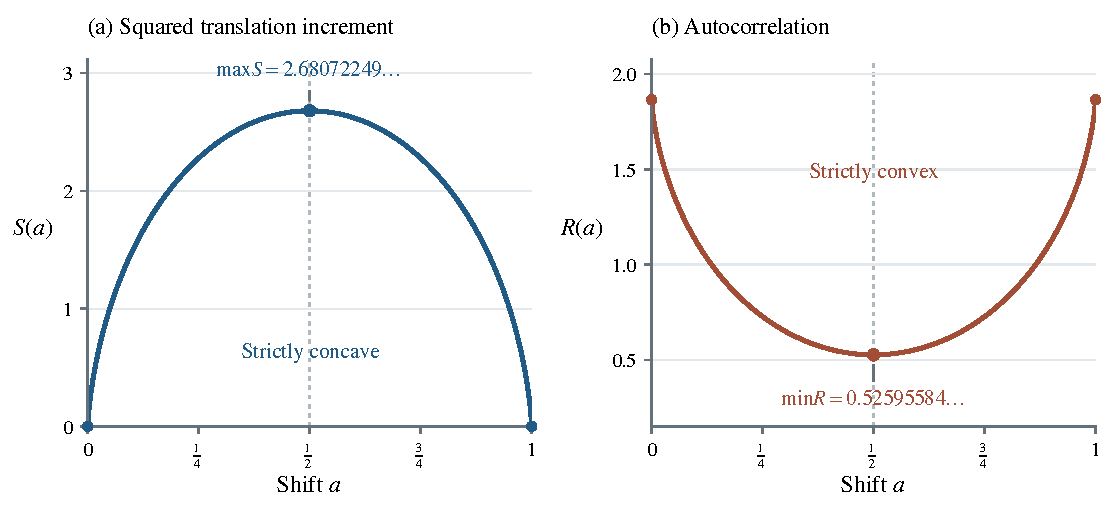
\includegraphics[width=\textwidth]{figures/gamma_correlation_figure.pdf}
\caption{Periodic log-Gamma correlations. The squared translation increment
$S(a)$ is strictly concave, and the autocorrelation $R(a)=R(0)-S(a)/2$
is strictly convex. The dashed guides mark the unique interior extrema at
$a=1/2$. The curves use the convergent series of
Theorem~\ref{gamma:thm:loggamma-concavity} and analytic endpoint limits;
the shape assertions are proved above.}
\label{gamma:fig:correlation}
\end{figure}

\begin{corollary}[Sharp endpoint expansion]
\label{gamma:cor:sharp-cusp}
As $a\downarrow0$,
\begin{align}
 S(a)={}&a\left[\log^2\frac1a+2\log\frac1a+2+\frac{\pi^2}{3}\right]
       +\left(2\gamma_1-\frac{\pi^2}{3}\right)a^2\notag\\
 &-\frac{a^4}{3}\left[\frac32\zeta(3)+\zeta'(3)\right]+O(a^6).
 \label{gamma:eq:sharp-cusp}
\end{align}
The leading behavior is $S(a)\sim a\log^2(1/a)$, with the full
coefficient polynomial and the first analytic corrections explicit.
\end{corollary}

\begin{corollary}[Effective truncation]
\label{gamma:cor:tail}
Let $S_N(a)$ be the right side of
\eqref{gamma:eq:loggamma-increment-series} truncated after $j=N$, where
$N\ge2$. Then
\begin{equation}
 0<S_N(a)-S(a)
 \le\frac{2\zeta(3)[1+\log(2N+2)]}{(N+1)^2}
             \frac{a^{2N+2}}{1-a^2}.
 \label{gamma:eq:tail-bound}
\end{equation}
By symmetry one can always replace $a$ by $\min(a,1-a)\le1/2$ before
evaluating this series.
\end{corollary}

\begin{proof}
The omitted coefficients have one sign. For $j\ge2$,
\[
 0<H_{2j-2}\zeta(2j-1)+\zeta'(2j-1)
    <\zeta(3)[1+\log(2j)],
 \qquad j(2j-1)\ge j^2.
\]
The function $(1+\log(2x))/x^2$ decreases for $x\ge1$.
Majorizing it at $x=N+1$ and summing the geometric tail proves
\eqref{gamma:eq:tail-bound}.
\end{proof}

\subsection{The extremal half-shift and a geometric zeta identity}

\begin{corollary}[Exact maximum]
\label{gamma:cor:half-maximum}
Let $q=\log2$ and $A=\gamma+\log(2\pi)$. Then
\begin{equation}
 \begin{split}
 S(1/2)={}&\frac{3\zeta''(2)+2(q-3A)\zeta'(2)}{2\pi^2}
       +\frac{A^2}{4}-\frac{Aq}{6}-\frac{q^2}{12}+\frac{\pi^2}{16}\\
 ={}&2.68072248798050738482152413952\ldots .
 \end{split}
 \label{gamma:eq:half-maximum}
\end{equation}
Equating this value with the convergent shift expansion gives
\begin{equation}
 \sum_{j=2}^{\infty}\frac{2[H_{2j-2}\zeta(2j-1)+\zeta'(2j-1)]}
                  {4^j j(2j-1)}
 =1+\log2+\frac{\log^2 2}{2}+\frac{\pi^2}{12}
              +\frac{\gamma_1}{2}-S(1/2).
 \label{gamma:eq:dyadic-series}
\end{equation}
\end{corollary}

\begin{proof}
In \eqref{gamma:eq:R-polylog}, use
$\Li_w(-1)=(2^{1-w}-1)\zeta(w)$. Hence
\[
 S(1/2)=\left.\frac1{\pi^2}
   \left[(\partial_w-A)^2+\frac{\pi^2}{4}\right]
       [(2-2^{1-w})\zeta(w)]\right|_{w=2}.
\]
At $w=2$, the three derivatives of $2-2^{1-w}$ required here are
$3/2$, $q/2$, and $-q^2/2$. Expanding and using $\zeta(2)=\pi^2/6$
proves \eqref{gamma:eq:half-maximum}. Substitution of $a=1/2$ into
\eqref{gamma:eq:loggamma-increment-series} proves
\eqref{gamma:eq:dyadic-series}.
\end{proof}

\section{Balanced negative polygamma correlations}
\label{gamma:sec:negative-polygamma}

For an integer $m\ge1$, define the classical balanced normalization
\begin{equation}
 \Psi_m(x)=\frac{\zeta'(1-m,x)+H_{m-1}\zeta(1-m,x)}{(m-1)!}.
 \label{gamma:eq:balanced}
\end{equation}
This is the Espinosa--Moll balanced negapolygamma
\cite{gamma:EspinosaMoll2004}. In particular
$\Psi_1=J_1=g-\ell/2$. It differs from the zero-based repeated
integrals of $g$ used elsewhere in the manuscript by explicit
polynomials. The normalization must be specified before periodizing:
polynomial changes can change endpoint jumps and Fourier decay.

For $m\ge2$, $\Psi_m'=\Psi_{m-1}$,
$\int_0^1\Psi_m=0$, and the endpoint values match.
The same mean-zero assertion holds for $m=1$, whose left endpoint is
logarithmically singular. These facts follow directly from the Hurwitz
shift and derivative identities.

\begin{theorem}[One polylogarithmic operator for the integrated tower]
\label{gamma:thm:balanced-correlation}
For all integers $m,n\ge1$ and $0<a<1$,
\begin{equation}
 \begin{split}
 &\int_0^1\Psi_m(x)\Psi_n(\{x+a\})\,dx\\
 &\quad=\frac2{(2\pi)^{m+n}}
 \Re\left[
    e^{\pi i(m-n)/2}
    \left((\partial_w-A)^2+\frac{\pi^2}{4}\right)
    \Li_w(e^{2\pi ia})\right]_{w=m+n},
 \qquad A=\gamma+\log(2\pi).
 \end{split}
 \label{gamma:eq:balanced-correlation}
\end{equation}
The zero-shift value is obtained by replacing $\Li_w$ with $\zeta(w)$.
At every rational shift, all terms reduce by a finite Fourier transform
to Hurwitz zeta values and their first two spectral derivatives at the
positive integer $m+n$.
\end{theorem}

\begin{proof}
Differentiate \eqref{gamma:eq:hurwitz-fourier} at $s=1-m$ and add the
$H_{m-1}$ multiple. Since
$\psi(m)=H_{m-1}-\gamma$, the harmonic numbers cancel, giving
\begin{equation}
 \widehat\Psi_m(k)
 =\frac{\gamma+\log(2\pi ik)}{(2\pi ik)^m},
 \qquad k\ne0;\qquad \widehat\Psi_m(0)=0.
 \label{gamma:eq:balanced-fourier}
\end{equation}
For $m=1$ this is interpreted in $L^2$; for $m\ge2$ the series is
absolutely convergent. Parseval's product formula therefore applies
in every case. For $k>0$, the product of the opposite-index
coefficients has modulus factor
$(A+\log k)^2+\pi^2/4$ and phase $e^{\pi i(n-m)/2}$.
Combining both signs of $k$ gives
\eqref{gamma:eq:balanced-correlation} because
$\partial_w k^{-w}=-(\log k)k^{-w}$.
The rational-shift statement follows by twice differentiating
\[
 \Li_w(e^{2\pi ip/q})
    =q^{-w}\sum_{r=1}^q e^{2\pi ipr/q}\zeta(w,r/q).
\]
\end{proof}

\begin{corollary}[Exact regularity threshold]
\label{gamma:cor:sobolev}
The periodized function $\Psi_m$ belongs to the circle Sobolev space
$H^\sigma$ exactly when $\sigma<m-1/2$. More generally, for any
$k,r\ge0$, the periodized function
$x\mapsto\partial_s^r\zeta(-k,x)$ belongs to $H^\sigma$ exactly when
$\sigma<k+1/2$.
\end{corollary}

\begin{proof}
With the Fourier definition
$\|f\|_{H^\sigma}^2\asymp\sum_k(1+k^2)^\sigma|\widehat f(k)|^2$,
\eqref{gamma:eq:balanced-fourier} reduces the first claim to convergence
of $\sum_{k\ge2}k^{2\sigma-2m}\log^2k$.
For a general spectral jet, differentiating
\eqref{gamma:eq:hurwitz-fourier} gives
\[
 |\widehat{\partial_s^r\zeta(-k,\cdot)}(n)|
 \sim\frac{k!}{(2\pi)^{k+1}}
              \frac{(\log n)^r}{n^{k+1}}\qquad(n\to+\infty),
\]
with the same power law at negative frequencies.
The comparison series converges exactly below the stated threshold,
including divergence at equality.
\end{proof}

\begin{remark}[Boundary of ordinary integral formulas]
\label{gamma:rem:boundary}
The restriction $m,n\ge1$ in
Theorem~\ref{gamma:thm:balanced-correlation} is essential. The next
derivative is the ordinary digamma function, with a $1/x$ singularity;
periodic shifted products containing it need an explicitly prescribed
finite-part or distributional interpretation. The absolutely
convergent integral theorem does not silently provide such a
regularization.
\end{remark}

% Self-contained contribution. Standard AMS theorem environments and macros
% \Li, \dd, \E, \Re are supplied by the parent document.
% Bibliography keys used: herg:RadchenkoZagier, herg:DLMFhyperbolic,
% herg:DLMFbessel, herg:DLMFgamma, herg:DLMFzeta.

\section{A uniform transition for high Herglotz derivatives}
\label{herg:sec:transition}

The frozen manuscript proves a sharp asymptotic expansion for the
Herglotz derivatives when their order tends to infinity at a fixed
positive argument \cite{repoHerglotz}. Its final research paragraph explicitly leaves open
a joint limit in which the argument also varies. We resolve the
transition scale $x\asymp r$. The result has a complete expansion with
computable coefficients, an explicit finite-order remainder, and a
profile that admits arithmetic, Bessel, Gamma, and dilogarithmic
representations. The special-function identities used in the proof are
classical; the contribution here is the joint-limit theorem and its
systematic connection to this profile. No historical priority is claimed
for an isolated transformed divisor sum.

Let
\begin{equation}\label{herg:eq:F}
 F(x)=\sum_{n\geq1}\frac{\psi(nx)-\log(nx)}{n},\qquad
 D_r(x)=\frac{(-1)^{r+1}x^{r+1}}{r!}F^{(r)}(x),
 \quad x>0,\quad r\geq1.
\end{equation}
Here $F^{(r)}$ differentiates the argument $x$. Define
\begin{equation}\label{herg:eq:Bprofile}
 B(t)=\frac{1}{1-e^{-t}}-\frac1t,\qquad B(0)=\frac12,
 \qquad
 S(\lambda)=\sum_{n\geq1}\frac1{n^2}
                       B\left(\frac1{n\lambda}\right),\quad\lambda>0.
\end{equation}
The letter $B$ without an index denotes this elementary function;
$B_j$ with an integer index denotes a Bernoulli number.

\subsection{An exact probability representation and a finite remainder}

\begin{lemma}[Positive kernel and derivative bounds]
\label{herg:lem:B}
For $t>0$, $1/2<B(t)<1$ and $B'(t)>0$. For every integer $q\geq1$,
\begin{equation}\label{herg:eq:Bbound}
 \sup_{t\geq0}|B^{(q)}(t)|
 \leq \frac{2q!\zeta(q+1)}{(2\pi)^{q+1}}.
\end{equation}
\end{lemma}
\begin{proof}
The hyperbolic partial-fraction expansion
\cite[Eq.~4.36.3]{herg:DLMFhyperbolic} gives
\begin{equation}\label{herg:eq:Bpartial}
 B(t)=\frac12+2t\sum_{m\geq1}\frac1{t^2+4\pi^2m^2}
 =\frac12+\sum_{m\geq1}
       \left(\frac1{t-2\pi im}+\frac1{t+2\pi im}\right).
\end{equation}
The second sum is paired as displayed. For $q\geq1$, differentiating
gives an absolutely and uniformly convergent series on the real axis;
$|t\pm2\pi im|\geq2\pi m$ proves \eqref{herg:eq:Bbound}.
Furthermore,
\[
 B'(t)=\frac1{t^2}-\frac1{4\sinh^2(t/2)}>0,
\]
since $\sinh(t/2)>t/2$. The limits at zero and infinity are $1/2$
and $1$, respectively. The derivative bound is asserted only for
$q\geq1$; its displayed right-hand side would be divergent at $q=0$.
\end{proof}

Let $Y_r$ have the gamma density
\begin{equation}\label{herg:eq:Ydensity}
 \frac{r^{r+1}}{r!}y^r e^{-ry},\qquad y>0,
\end{equation}
and put
\begin{equation}\label{herg:eq:moments}
 \mu_m(r)=\E(Y_r-1)^m
 =\sum_{\ell=0}^m(-1)^{m-\ell}\binom m\ell
                         \frac{(r+1)_\ell}{r^\ell}.
\end{equation}
Each $\mu_m(r)$ is an exact polynomial in $r^{-1}$; it need not be
evaluated by subtracting floating-point numbers.

\begin{theorem}[Exact mixture and computable Taylor certificate]
\label{herg:thm:mixture}
For all $r\geq1$ and $\lambda>0$,
\begin{equation}\label{herg:eq:mixture}
 D_r(r\lambda)=\E S(\lambda/Y_r).
\end{equation}
Write $h_\lambda(y)=S(\lambda/y)$ for $y>0$, extended by
$h_\lambda(0)=\zeta(2)/2$. For $J\geq0$ and $q=2J+2$,
\begin{align}
 &\left|D_r(r\lambda)-
   \sum_{m=0}^{2J+1}\frac{h_\lambda^{(m)}(1)}{m!}\mu_m(r)\right|
 \label{herg:eq:certificate}\\[-2pt]
 &\hspace{18mm}\leq
 \frac{2\zeta(q+1)\zeta(q+2)}{(2\pi)^{q+1}\lambda^q}\mu_q(r).
 \notag
\end{align}
This is a finite-$r$ inequality, valid on the entire positive
$\lambda$ axis, rather than an unspecified asymptotic error.
\end{theorem}
\begin{proof}
The classical digamma integral, also used in the Herglotz theory of
Radchenko--Zagier \cite{herg:RadchenkoZagier}, is
\[
 \psi(z)-\log z=-\int_0^\infty e^{-zt}B(t)\,\dd t,
 \qquad z>0.
\]
Since $0<B<1$, the defining sum and any fixed number of its
argument derivatives converge locally uniformly. Differentiating and
substituting $u=nxt$ gives
\begin{equation}\label{herg:eq:pre-mixture}
 D_r(x)=\sum_{n\geq1}\frac1{n^2r!}
           \int_0^\infty u^r e^{-u}B\left(\frac{u}{nx}\right)\dd u.
\end{equation}
All integrands are positive and bounded after normalization by the
summable sequence $n^{-2}$. Thus every interchange is justified, and
$x=r\lambda$ proves \eqref{herg:eq:mixture}.

From \eqref{herg:eq:Bbound}, for every $q\geq1$,
\[
 \sup_{y\geq0}|h_\lambda^{(q)}(y)|
 \leq \frac{2q!\zeta(q+1)\zeta(q+2)}
                    {(2\pi)^{q+1}\lambda^q}.
\]
Taylor's formula at $y=1$, through degree $q-1$, therefore has a
global remainder bounded by the last constant times $|y-1|^q/q!$.
Taking expectations proves \eqref{herg:eq:certificate}, because $q$
is even. Formula \eqref{herg:eq:moments} follows from the elementary
gamma moments.
\end{proof}

\subsection{The complete expansion and its scope}

Define the finite polynomials $C_j(z)=\sum_m c_{j,m}z^m$ by
\begin{equation}\label{herg:eq:C}
 \sum_{j\geq0}C_j(z)w^j
 =\exp\left\{\sum_{\ell\geq1}w^\ell
          \left(\frac{z^\ell}{\ell}
                       +\frac{z^{\ell+1}}{\ell+1}\right)\right\}.
\end{equation}
Thus $\deg C_j\leq2j$. Let $\mathcal E=\lambda\,\mathrm d/\mathrm d\lambda$
and use the rising operator factorial
$\mathcal E^{\overline m}=\mathcal E(\mathcal E+1)\cdots
(\mathcal E+m-1)$, with value $1$ at $m=0$. Put
\begin{equation}\label{herg:eq:T}
 \mathcal T_j=
   \sum_m c_{j,m}(-1)^m\mathcal E^{\overline m}.
\end{equation}
This definition specifies every coefficient without an implicit
recurrence for special-function values.

\begin{theorem}[Uniform complete transition expansion]
\label{herg:thm:expansion}
For any nonnegative integers $J,u$ and any compact interval
$I\subset(0,\infty)$,
\begin{equation}\label{herg:eq:expansion}
 D_r(r\lambda)=\sum_{j=0}^J\frac{(\mathcal T_jS)(\lambda)}{r^j}
                +O_{I,J,u}(r^{-J-1}),\qquad r\longrightarrow\infty,
\end{equation}
uniformly for $\lambda\in I$, also after up to $u$ derivatives in
$\lambda$. In particular,
\begin{align}
 D_r(r\lambda)={}&S(\lambda)
  +\frac{\lambda^2S''(\lambda)}{2r}\label{herg:eq:firstcoeffs}\\
 &+\frac1{r^2}
 \left(\frac{\lambda^2S''(\lambda)}2
       +\frac{2\lambda^3S'''(\lambda)}3
       +\frac{\lambda^4S^{(4)}(\lambda)}8\right)+O_I(r^{-3}).\notag
\end{align}
\end{theorem}
\begin{proof}
The exact moment generating function is
\[
 \E e^{z(Y_r-1)}=e^{-z}(1-z/r)^{-r-1}.
\]
Its logarithm expands as the exponent in \eqref{herg:eq:C} with
$w=r^{-1}$. Therefore the coefficient of $r^{-j}$ in
$\mu_m(r)/m!$ is $[z^m]C_j(z)$. In particular
$\mu_{2J+2}(r)=O_J(r^{-J-1})$. The finite Taylor certificate proves
the complete expansion, since all central moments in it are exact
polynomials. Finally,
\[
 h_\lambda^{(m)}(1)=(-1)^m\mathcal E^{\overline m}S(\lambda),
\]
which follows by induction on $m$, proves \eqref{herg:eq:T}.

For derivative uniformity, apply the same argument to each fixed
$\partial_\lambda^v h_\lambda$. For $b\geq1$ the function
$t^bB^{(b)}(t)$ is bounded on $[0,\infty)$, by regularity at zero
and the elementary large-$t$ form $B(t)=1-t^{-1}+O(e^{-t})$.
Thus the required parameter derivatives may also be passed through
the expectation and the $n$ sum. A mixed derivative is a finite sum
of terms involving $t^bB^{(q+b)}(t)$, with $q=2J+2\geq2$.
Differentiating the paired fractions in \eqref{herg:eq:Bpartial} gives
\[
 \sup_{t\geq0}|t^b B^{(q+b)}(t)|
 \leq\frac{2(q+b)!\zeta(q+1)}{(2\pi)^{q+1}}.
\]
Indeed $t^b\leq|t\pm2\pi im|^b$. The remaining powers of
$n^{-1}$ are summable and $\lambda^{-1}$ is bounded on $I$.
This supplies the required uniform Taylor remainders after each
parameter differentiation. No uncontrolled big-$O$ term is differentiated.

For the displayed coefficients,
$C_1(z)=z+z^2/2$ and
$C_2(z)=z^2+5z^3/6+z^4/8$; substituting into
\eqref{herg:eq:T} gives \eqref{herg:eq:firstcoeffs}.
\end{proof}

\begin{corollary}[All limiting ratios and noncommuting limits]
\label{herg:cor:ratios}
The function $S$ is strictly decreasing, with
\[
 \lim_{\lambda\downarrow0}S(\lambda)=\zeta(2),\qquad
 \lim_{\lambda\to\infty}S(\lambda)=\frac{\zeta(2)}2.
\]
If $r\to\infty$ through integers and $x_r/r\to\lambda$ in the
extended interval $[0,\infty]$, then $D_r(x_r)$ tends to the
corresponding value of this continuously extended profile.
Consequently,
\[
 \lim_{x\to\infty}\lim_{r\to\infty}D_r(x)=\zeta(2),\qquad
 \lim_{r\to\infty}\lim_{x\to\infty}D_r(x)=\frac{\zeta(2)}2.
\]
The complete correction expansion is claimed on compact positive
ratio intervals; the two endpoint statements concern the leading
limit only.
\end{corollary}
\begin{proof}
Strict monotonicity follows termwise from $B'>0$. Dominated
convergence, using $1/2\leq B\leq1$, proves the limits of $S$.
Moreover $Y_r\to1$ in probability, since
$\E(Y_r-1)^2=r^{-1}+2r^{-2}$. In \eqref{herg:eq:pre-mixture}
each fixed-$n$ argument consequently tends in probability to
$1/(n\lambda)$, to infinity, or to zero, according to the ratio.
Bounded convergence in probability and the summable $n^{-2}$ bound
give the asserted three cases. At fixed $r$, letting $x\to\infty$
in \eqref{herg:eq:pre-mixture} gives $\zeta(2)/2$ directly.
\end{proof}

\section{Arithmetic continuation and zeros of the centered profile}
\label{herg:sec:profile}

Write $\sigma_{-1}(N)=\sum_{d\mid N}d^{-1}$. This section gives
exact formulas for the function that enters the joint-limit theorem,
including the complex zeros of its centered reciprocal form
$H(y)-\zeta(2)/2$. These are zeros of that centered function, not
zeros of $S$, $H$, or the original generalized Stieltjes constants.

\begin{theorem}[Arithmetic representation and meromorphic zeros]
\label{herg:thm:profilezeros}
For $\lambda>0$,
\begin{equation}\label{herg:eq:divisorprofile}
 S(\lambda)=\frac{\zeta(2)}2+
       2\lambda\sum_{N\geq1}
              \frac{\sigma_{-1}(N)}{1+4\pi^2N^2\lambda^2}.
\end{equation}
The reciprocal profile $H(y)=S(1/y)$ extends meromorphically to
the complex plane by
\begin{equation}\label{herg:eq:Hpartial}
 H(y)=\frac{\zeta(2)}2+
           2y\sum_{N\geq1}
                       \frac{\sigma_{-1}(N)}{y^2+4\pi^2N^2}.
\end{equation}
It has simple poles at $y=\pm2\pi iN$, of residue
$\sigma_{-1}(N)$. The zeros of $H(y)-\zeta(2)/2$ are precisely
the simple zero $y=0$ and the simple pairs $y=\pm i b_N$, where
there is exactly one $b_N$ in every interval
\begin{equation}\label{herg:eq:zerointervals}
 2\pi N<b_N<2\pi(N+1),\qquad N\geq1.
\end{equation}
There are no other zeros. In particular, every nonzero zero is
purely imaginary and strictly interlaces with the poles.
\end{theorem}
\begin{proof}
Insert \eqref{herg:eq:Bpartial} into \eqref{herg:eq:Bprofile}.
All terms are positive for positive arguments, so rearrangement is
permitted. Grouping the pair $(m,n)$ by $N=mn$ gives
\eqref{herg:eq:divisorprofile}. Since
$\sigma_{-1}(N)\leq1+\log N$, the series in
\eqref{herg:eq:Hpartial} converges locally uniformly away from its
displayed poles, and direct residue calculation gives their residues.

Put
\[
 T(z)=\sum_{N\geq1}\frac{\sigma_{-1}(N)}{z+4\pi^2N^2},
 \qquad H(y)-\zeta(2)/2=2yT(y^2).
\]
For nonreal $z$,
\[
 \Im T(z)=-(\Im z)\sum_{N\geq1}
             \frac{\sigma_{-1}(N)}{|z+4\pi^2N^2|^2}\ne0.
\]
For real $z>-4\pi^2$, $T(z)>0$. On each interval
$(-4\pi^2(N+1)^2,-4\pi^2N^2)$ the derivative
$T'(z)=-\sum\sigma_{-1}(j)/(z+4\pi^2j^2)^2$ is strictly
negative, while its endpoint limits are $+\infty$ and $-\infty$.
There is therefore exactly one simple zero in each interval and
none elsewhere. Taking square roots proves \eqref{herg:eq:zerointervals}.
Finally $H'(0)=2T(0)=\zeta(3)/12>0$, so the zero at the origin
is simple as well.
\end{proof}

The same representation gives positive moment and quadrature
structures. For example, for $v>0$,
\[
 \frac{S(\sqrt v)-\zeta(2)/2}{2\sqrt v}
 =\sum_{N\geq1}\frac{\sigma_{-1}(N)}{1+4\pi^2N^2v}
\]
is completely monotone in $v$: each derivative has the required
alternating sign, and the differentiated series converges locally
uniformly. This is a direct property of the displayed positive
discrete measure.

\subsection{Two complementary exact representations}

\begin{theorem}[Convergent zeta series and dual Bessel series]
\label{herg:thm:dual}
For $\lambda>1/(2\pi)$,
\begin{equation}\label{herg:eq:zetaprofile}
 S(\lambda)=\frac{\zeta(2)}2+
       \sum_{m\geq1}\frac{B_{2m}\zeta(2m+1)}{(2m)!\lambda^{2m-1}},
\end{equation}
an absolutely convergent series. For every $\lambda>0$, put
$R(\lambda)=S(\lambda)-\zeta(2)-\lambda(\log\lambda-\gamma)$.
Then
\begin{equation}\label{herg:eq:Besselprofile}
 R(\lambda)=4\lambda\sum_{N\geq1}\sigma_{-1}(N)
 \Re\left[
  \sqrt{\frac{2\pi iN}{\lambda}}\,
  K_1\left(2\sqrt{\frac{2\pi iN}{\lambda}}\right)\right],
\end{equation}
with principal square roots. The series is absolutely convergent and
locally uniformly convergent on the positive $\lambda$ axis.
\end{theorem}
\begin{proof}
The Taylor expansion of $B(t)$ at zero has radius $2\pi$.
Substitute it in \eqref{herg:eq:Bprofile}; absolute convergence
when $1/\lambda<2\pi$ gives \eqref{herg:eq:zetaprofile}.

For the second identity, Mellin inversion of $(1+u^2)^{-1}$ in
\eqref{herg:eq:divisorprofile} gives, for $1<c<2$,
\begin{equation}\label{herg:eq:Mellin}
 S(\lambda)-\frac{\zeta(2)}2
 =\frac1{2\pi i}\int_{c-i\infty}^{c+i\infty}
   \frac{\pi\zeta(s)\zeta(s+1)}{\sin(\pi s/2)}
       (2\pi)^{-s}\lambda^{1-s}\,\dd s.
\end{equation}
On this line the Dirichlet series is absolutely convergent; the
sine denominator supplies exponential vertical decay. Move the
line to $\Re s=-A$, with any fixed $A>1$. The only poles crossed
are $s=1$ and $s=0$. The negative even sine poles are cancelled
by the trivial zeros of $\zeta(s)$. Standard vertical-strip bounds
for zeta and the exponential factor justify the horizontal limits.
The residue at $1$ is $\zeta(2)/2$. At zero use
$\zeta(0)=-1/2$, $\zeta'(0)=-\frac12\log(2\pi)$, and
$\zeta(1+s)=s^{-1}+\gamma+O(s)$; the residue is
$\lambda(\log\lambda-\gamma)$.

The zeta functional equation \cite{herg:DLMFzeta}, applied twice,
transforms the remaining integral into
\begin{equation}\label{herg:eq:dualMellin}
 R(\lambda)=\frac{2\lambda}{2\pi i}\int_{(A)}
  \Gamma(w)\Gamma(w+1)\zeta(w)\zeta(w+1)
  \cos(\pi w/2)\left(\frac\lambda{2\pi}\right)^w\,\dd w.
\end{equation}
Here $\zeta(w)\zeta(w+1)=\sum\sigma_{-1}(N)N^{-w}$ is
absolutely convergent, and the product of the two gamma factors
and the cosine decays exponentially on the line. Termwise
integration is consequently justified. The standard Bessel
Mellin--Barnes formula \cite[Eq.~10.32.13]{herg:DLMFbessel} gives
\[
 \frac1{2\pi i}\int_{(A)}\Gamma(w)\Gamma(w+1)z^{-w}\,\dd w
       =2\sqrt z\,K_1(2\sqrt z),\qquad |\arg z|<\pi.
\]
Taking the average of its values at $z=2\pi iN/\lambda$ and
its conjugate produces the cosine factor and proves
\eqref{herg:eq:Besselprofile}.

For an explicit domination, set $v_N=2\sqrt{\pi N/\lambda}$.
The real-line Bessel integral implies
$|K_1(w)|\leq K_1(\Re w)\leq K_{3/2}(\Re w)$ for
$\Re w>0$. The last inequality follows from
$\cosh t\leq\cosh(3t/2)$ in that integral. Hence the absolute
value of the $N$th summand in \eqref{herg:eq:Besselprofile} is at most
\begin{equation}\label{herg:eq:sectorbound}
 2^{3/2}\pi^{3/4}\lambda^{3/4}\sigma_{-1}(N)N^{1/4}
                       e^{-v_N}(1+v_N^{-1}).
\end{equation}
This proves absolute and local uniform convergence independently
of the contour interchange.
\end{proof}

\begin{remark}[A simple numerical tail certificate]
\label{herg:rem:Besseltail}
Put $a=2\sqrt{\pi/\lambda}$ and
$C=2^{3/2}\pi^{3/4}\lambda^{3/4}$. For an integer cutoff $N\geq1$
with $a\sqrt N\geq3/2$, the absolute tail in
\eqref{herg:eq:Besselprofile} is bounded by
\begin{equation}\label{herg:eq:Besseltail}
 4C\left(1+\frac1{a\sqrt N}\right)a^{-7/2}
                  \Gamma\left(\frac72,a\sqrt N\right),
\end{equation}
where the final Gamma is the upper incomplete gamma function.
Indeed $\sigma_{-1}(n)\leq1+\log n\leq2\sqrt n$ for $n\geq1$,
and $t^{3/4}e^{-a\sqrt t}$ is decreasing for $a\sqrt t\geq3/2$.
Use the integral test and substitute $u=a\sqrt t$.
\end{remark}

\begin{corollary}[An exponentially small profile correction]
\label{herg:cor:smallratio}
As $\lambda\downarrow0$, let
\[
 A(\lambda)=2^{5/4}\pi^{3/4}\lambda^{3/4}
                       e^{-2\sqrt{\pi/\lambda}},\qquad
 \phi(\lambda)=2\sqrt{\pi/\lambda}-\frac\pi8.
\]
Then
\begin{equation}\label{herg:eq:smallratio}
 R(\lambda)=A(\lambda)
 \left[\cos\phi(\lambda)
 +\frac3{16}\sqrt{\frac\lambda{2\pi}}
       \cos\left(\phi(\lambda)+\frac\pi4\right)+O(\lambda)\right].
\end{equation}
This is additive; no division by a cosine near a zero is intended.
There are complete further powers of $\sqrt\lambda$, supplied by
the classical $K_1$ expansion. In particular $R$ takes both signs
arbitrarily close to zero.
\end{corollary}
\begin{proof}
In the $N=1$ sector, use the standard large-argument expansion
\cite[Eq.~10.40.2]{herg:DLMFbessel}
\[
 K_1(2\sqrt z)=\frac{\sqrt\pi}{2z^{1/4}}e^{-2\sqrt z}
        \left[1+\frac3{16\sqrt z}+O(z^{-1})\right]
\]
on the ray $\arg z=\pi/2$. Taking its real part gives exactly
\eqref{herg:eq:smallratio}. From \eqref{herg:eq:sectorbound},
the aggregate of the sectors $N\geq2$ is
$O(\lambda^{3/4}e^{-2\sqrt{2\pi/\lambda}})$: factor out its
$N=2$ exponential and dominate the remaining series at any fixed
positive lower value of $2\sqrt{\pi/\lambda}$. This is smaller
than every algebraic correction in the first sector. The phase
passes through arbitrarily large multiples of $\pi$ as
$\lambda\downarrow0$, proving the sign assertion.
\end{proof}

\section{Gamma and dilogarithm antiderivatives of the profile}
\label{herg:sec:primitives}

The profile admits convergent primitive identities in which the
subtractions are essential. They also provide useful test cases for
symbolic integration across the Gamma and polylogarithmic descriptions.

\begin{theorem}[Two normalized primitives]
\label{herg:thm:primitives}
For $y\geq0$ define
\begin{align}
 G(y)&=-\sum_{n\geq1}\frac1n
   \log\left[\Gamma\left(1+\frac{iy}{2\pi n}\right)
             \Gamma\left(1-\frac{iy}{2\pi n}\right)\right],
 \label{herg:eq:Gprimitive}\\
 P(y)&=\sum_{n\geq1}\left\{
     \Li_2(e^{-y/n})-\zeta(2)-\frac yn\log\frac yn
                 +\frac yn+\frac{y^2}{4n^2}\right\},
 \label{herg:eq:Pprimitive}
\end{align}
where terms at $y=0$ are taken by continuity. Each Gamma product is
strictly positive, so its logarithm is the real logarithm. Both
series converge locally uniformly, with the derivatives needed below,
and
\begin{equation}\label{herg:eq:primitivechain}
 P'(y)=G(y),\qquad G'(y)=P''(y)=H(y)-\frac{\zeta(2)}2,
 \qquad P(0)=P'(0)=G(0)=0.
\end{equation}
Equivalently,
\begin{equation}\label{herg:eq:Gammameasureprimitive}
 \int_\lambda^\infty
     \frac{S(u)-\zeta(2)/2}{u^2}\,\dd u=G(1/\lambda),
 \qquad\lambda>0.
\end{equation}
For $|y|<2\pi$ the corresponding convergent zeta-product series are
\begin{align}
 G(y)&=\sum_{m\geq1}
  \frac{B_{2m}\zeta(2m+1)}{(2m)!(2m)}y^{2m},
 \label{herg:eq:Gseries}\\
 P(y)&=\sum_{m\geq1}
  \frac{B_{2m}\zeta(2m+1)}{(2m)!(2m)(2m+1)}y^{2m+1}.
 \label{herg:eq:Pseries}
\end{align}
For example,
\[
 G(y)=\frac{\zeta(3)}{24}y^2-\frac{\zeta(5)}{2880}y^4+\cdots,
 \qquad
 P(y)=\frac{\zeta(3)}{72}y^3-\frac{\zeta(5)}{14400}y^5+\cdots.
\]
\end{theorem}
\begin{proof}
The reflection formula and the gamma recurrence
\cite[\S5.5]{herg:DLMFgamma} give, for $t\geq0$,
\[
 \Gamma\left(1+\frac{it}{2\pi}\right)
 \Gamma\left(1-\frac{it}{2\pi}\right)
     =\frac{t/2}{\sinh(t/2)}.
\]
Consequently the function
\[
 L(t)=\log\frac{\sinh(t/2)}{t/2}
      =\frac t2+\log(1-e^{-t})-\log t
\]
satisfies $L(0)=0$ and $L'(t)=B(t)-1/2$. Its primitive vanishing
at zero is
\[
 J(t)=\Li_2(e^{-t})-\zeta(2)-t\log t+t+\frac{t^2}4,
 \qquad J'(t)=L(t).
\]
Indeed $\mathrm d\Li_2(e^{-t})/\mathrm dt=\log(1-e^{-t})$.
Now $G(y)=\sum n^{-1}L(y/n)$ and $P(y)=\sum J(y/n)$.
Since $L(t)=O(t^2)$, $J(t)=O(t^3)$, and their requisite
derivatives have the corresponding bounds at zero, the series and
their stated derivatives converge uniformly on bounded positive
$y$ intervals. This proves all of \eqref{herg:eq:primitivechain}.
The substitution $y=1/u$ proves
\eqref{herg:eq:Gammameasureprimitive}. Termwise integration of the
Taylor series for $H(y)-\zeta(2)/2$ proves
\eqref{herg:eq:Gseries}--\eqref{herg:eq:Pseries}.
\end{proof}

\paragraph{Further questions arising from this theorem.}
The complete expansion above suggests a uniform matching analysis when
$\lambda=\lambda_r\downarrow0$: one must compare its derivative-dependent
remainder with the exponentially small Bessel sectors before importing
fixed-$x$ oscillatory formulas. A second problem is the asymptotic
location of the imaginary zeros $b_N$ within their certified pole
intervals; their residues are the irregular but explicit divisor weights
$\sigma_{-1}(N)$. A third is to exploit the positive Stieltjes
representation for rational upper and lower approximants to $S$, then
combine them with the exact gamma-moment remainder. Finally, logarithmic
weights in the defining Herglotz sum should yield spectral derivatives
of the divisor Dirichlet series, with zeta derivatives and Laurent
coefficients entering the transformed residue terms. These are separate
extensions; none is presumed by the compact-ratio theorem proved here.

% Suggested bibliography entries (parent should place in its bibliography):
% \bibitem{herg:RadchenkoZagier} D. Radchenko and D. Zagier,
% ``Arithmetic properties of the Herglotz function'',
% arXiv:2012.15805, https://arxiv.org/abs/2012.15805.
% \bibitem{herg:DLMFhyperbolic} NIST DLMF, Sec. 4.36,
% https://dlmf.nist.gov/4.36 (especially Eq. 4.36.3).
% \bibitem{herg:DLMFbessel} NIST DLMF, Secs. 10.32 and 10.40,
% https://dlmf.nist.gov/10.32 and https://dlmf.nist.gov/10.40.
% \bibitem{herg:DLMFgamma} NIST DLMF, Sec. 5.5,
% https://dlmf.nist.gov/5.5 (reflection and recurrence).
% \bibitem{herg:DLMFzeta} NIST DLMF, Sec. 25.4,
% https://dlmf.nist.gov/25.4 (Riemann zeta functional equation).

\section{Nonseparable reflection jets: a two-generator theorem}
\label{ns:sec:jets}

The manuscript proves a multivariable product law when the active deformation
parameters are separate powers of coordinate variables. Its warning that a
general multivariable substitution requires the full Koszul complex is
essential. We now give a different sufficient condition: the ideal generated
by the active parameters may have arbitrary mixed terms, provided it needs at
most two generators. We also exhibit an explicit three-generator obstruction.
The results concern the specified formal distribution presentation. They do
not assert independence of evaluated polylogarithm or zeta values.

\subsection{The distribution presentation and the input theorem}

For an integer $q>2$, put $X_q=(q^{-1}\mathbb Z)/\mathbb Z$. Given weights
$a_p$ in a commutative coefficient ring $S$, one for each prime $p\mid q$,
define
\begin{equation}\label{ns:eq:distribution}
 \mathcal D_q(S,a)=
 \left(\bigoplus_{x\in X_q}S e_x\right)
 \Big/
 \left\langle
  \sum_{\substack{y\in X_q\\py=x}}e_y-a_pe_x:
  p\mid q,\ x\in X_{q/p}
 \right\rangle.
\end{equation}
Reflection acts by $ce_x=e_{-x}$. Write
\[
 n=\frac{\varphi(q)}2,\qquad
 r=\#\{p>2:p\mid q\}+\mathbf1_{4\mid q}.
\]
The active sequence is
\begin{equation}\label{ns:eq:active}
 \boldsymbol\delta=
 (a_p-1:p>2,\ p\mid q),
 \quad\text{with }a_2(a_2-1)\text{ appended if }4\mid q.
\end{equation}
There is no active entry at $2$ when $v_2(q)=1$.

We use the following established results from the frozen manuscript \cite{repoJets}.
The all-ring basis theorem makes $\mathcal D_q(S,a)$ free of rank
$\varphi(q)$. In characteristic two, with $N=c-1$, its reflection homology is
\begin{equation}\label{ns:eq:input-koszul}
 \ker N/\operatorname{im}N
 \simeq\bigoplus_{j=0}^r H_j(K_S(\boldsymbol\delta)).
\end{equation}
For a finite free $\mathbb Z$-algebra $B$, put $\overline B=B/2B$ and
$C_\pm=\mathcal D_q(B,a)/(c\mp1)\mathcal D_q(B,a)$. Then
\begin{align}
 \operatorname{Tor}_{\mathbb Z}C_+
 &\simeq\bigoplus_{j\ {
m odd}}
 H_j(K_{\overline B}(\overline{\boldsymbol\delta})),
 \label{ns:eq:input-plus}\\
 \operatorname{Tor}_{\mathbb Z}C_-
 &\simeq\bigoplus_{j\ {
m even}}
 H_j(K_{\overline B}(\overline{\boldsymbol\delta})).
 \label{ns:eq:input-minus}
\end{align}
Every integer-torsion class is killed by two, and both free abelian ranks are
$n\operatorname{rank}_{\mathbb Z}B$. The source labels are
\path{ir:thm:integral} in
\path{08-integral-02-integral.tex},
\path{ir:thm:char2-koszul} in
\path{08-integral-05-modular-jets.tex}, and
\path{irjet:thm:finite-free-koszul} in
\path{08-integral-jets.tex}. Thus the algebraic input and the new step below
are separately identifiable.

\subsection{A colength law without separated parameters}

A finite-dimensional commutative $k$-algebra $S$ is \emph{Frobenius} here if it
admits a $k$-linear functional $\tau:S\to k$ such that $(u,v)\mapsto\tau(uv)$
is a nondegenerate pairing. The rectangular jet algebra
\begin{equation}\label{ns:eq:rectangular}
 S=k[t_1,\ldots,t_d]/(t_1^{L_1},\ldots,t_d^{L_d}),\qquad L_i\ge1,
\end{equation}
is a local Frobenius algebra. Take $\tau$ to be the coefficient of
$t_1^{L_1-1}\cdots t_d^{L_d-1}$: complementary basis monomials pair to one.
Its dimension is $T=\prod_iL_i$.

\begin{theorem}[Two-generator colength law]\label{ns:thm:two-generator}
Let $S$ be a finite-dimensional commutative local Frobenius algebra over a
field $k$. Let $\boldsymbol f=(f_1,\ldots,f_r)$, with $r\ge1$, and suppose
that $I=(f_1,\ldots,f_r)$ can be generated by at most two elements. Put
$\ell=\dim_k(S/I)$. Then
\begin{equation}\label{ns:eq:binomial}
 \dim_k H_j(K_S(\boldsymbol f))=\binom rj\ell,
 \qquad 0\le j\le r.
\end{equation}
This statement holds in every characteristic.
\end{theorem}

\begin{proof}
If $I=S$, some entry is a unit because $S$ is local. Its two-term Koszul
factor is contractible, and both sides of \eqref{ns:eq:binomial} vanish.
If $I=0$, the differential is zero and the assertion is immediate.

Otherwise choose a minimal generating subset among the given entries.
One obtains it by choosing a basis of $I/\mathfrak mI$ from their residue
classes and applying Nakayama's lemma. This subset has at most two elements.
Permute those elements to the beginning of the list. Every remaining entry
is a linear combination of them, so elementary invertible operations change
the list into $(f,g,0,\ldots,0)$, allowing $g=0$ if only one generator is
needed. These operations induce isomorphisms on the free module defining
the Koszul complex and on all its exterior powers.

For $r=1$, the kernel and cokernel of the square linear map
$S\xrightarrow{f}S$ have the same dimension, proving the assertion. For
$r\ge2$, first consider the two-entry complex
\[
 0\longrightarrow S\longrightarrow S^2\longrightarrow S\longrightarrow0.
\]
Its zeroth homology is $S/I$, and its second homology is
$\operatorname{Ann}_S(I)$. The Frobenius pairing identifies
\begin{equation}\label{ns:eq:dual}
 \operatorname{Ann}_S(I)\simeq\operatorname{Hom}_k(S/I,k)
\end{equation}
as $S$-modules. Indeed, the orthogonal complement of $I$ is precisely its
annihilator. To see the nontrivial inclusion, suppose $\tau(zi)=0$ for
all $i\in I$. For every $a\in S$, one then has $\tau((zi)a)=0$, because
$ia\in I$. Nondegeneracy gives $zi=0$.

The two end homology groups therefore have dimension $\ell$. The Euler
characteristic of the complex is $T-2T+T=0$, so its middle homology has
dimension $2\ell$. Tensoring with the zero-differential exterior algebra
on the remaining $r-2$ generators yields
\[
 \dim_kH_j
 =\ell\left[\binom{r-2}j+2\binom{r-2}{j-1}
                  +\binom{r-2}{j-2}\right]
 =\ell\binom rj.
\]
No separability of the entries has been used.
\end{proof}

\begin{corollary}[Nonseparable reflection formula]\label{ns:cor:reflection}
Let $S$ be as in Theorem~\ref{ns:thm:two-generator}, now in characteristic
two, and put $T=\dim_kS$. If the active ideal generated by
\eqref{ns:eq:active} needs at most two generators, then
\begin{equation}\label{ns:eq:reflection}
 \dim_k\mathcal D_q(S,a)/(c-1)\mathcal D_q(S,a)
 =nT+2^{r-1}\ell.
\end{equation}
For
$B=\mathbb Z[t_1,\ldots,t_d]/(t_1^{L_1},\ldots,t_d^{L_d})$, if the reduced
active ideal in $S=B/2B$ has that property, both signs have the abelian-group
decomposition
\begin{equation}\label{ns:eq:smith}
 C_\pm\simeq\mathbb Z^{nT}\oplus
                  (\mathbb Z/2\mathbb Z)^{2^{r-1}\ell}.
\end{equation}
No splitting as $B$-modules is asserted.
\end{corollary}

\begin{proof}
Since $N^2=0$ in characteristic two, an elementary rank calculation gives
\[
 \dim_k\operatorname{coker}N
 =\frac{\dim_k\mathcal D_q(S,a)+
                \dim_k(\ker N/\operatorname{im}N)}2.
\]
The first dimension is $2nT$. Equations \eqref{ns:eq:input-koszul} and
\eqref{ns:eq:binomial} make the second $2^r\ell$, proving
\eqref{ns:eq:reflection}. For the integral assertion, both parity sums of
the binomial coefficients are $2^{r-1}$; apply
\eqref{ns:eq:input-plus}--\eqref{ns:eq:input-minus} and the stated free rank.
\end{proof}

In particular, when $r(q)=2$, this settles the dimension and abelian Smith
problem for \emph{every} active sequence over a rectangular jet algebra.
The number of deformation variables need not equal the active-prime count.
When $r(q)>2$, the same theorem applies whenever the extra active parameters
are redundant generators of the ideal.

\subsection{Mixed monomials and a module obstruction}

Take $S=k[x,y]/(x^L,y^M)$ and
\[
 I=(x^a,x^by^c),\qquad 1\le b<a\le L,\quad1\le c\le M.
\]
A quotient basis consists of the monomials $x^iy^j$ with $i<a$ and with
either $i<b$ or $j<c$. Consequently
\begin{equation}\label{ns:eq:mixed-colength}
 \ell=bM+(a-b)c.
\end{equation}
This includes boundary cases where one displayed monomial is zero in $S$.
For two active parameters, the reflected dimension is therefore
\[
 nLM+2\bigl[bM+(a-b)c\bigr].
\]

For a concrete integral example, let $q=15$,
$B=\mathbb Z[x,y]/(x^3,y^3)$, and take
\[
 a_3=1+x^2,\qquad a_5=1+xy.
\]
Here $T=9$, $r=2$, $n=4$, and $\ell=4$. Thus
\begin{equation}\label{ns:eq:fifteen}
 C_\pm\simeq\mathbb Z^{36}\oplus(\mathbb Z/2\mathbb Z)^8,
 \qquad
 \dim_{\mathbb F_2}\mathcal D_{15}(S,a)/(c-1)=44.
\end{equation}

The module statement of the manuscript's separable product law does not
extend by replacing its quotient with an arbitrary $S/I$. In this example,
put $Q=S/(x^2,xy)$, over $k=\mathbb F_2$. Direct monomial calculation gives
\begin{align*}
 Q&:\quad 1,x,y,y^2,\\
 \operatorname{Ann}_S(I)&=(x^2,xy^2):\quad
             x^2,x^2y,x^2y^2,xy^2.
\end{align*}
The first module is cyclic. The second needs two generators: modulo
$\mathfrak m\operatorname{Ann}_S(I)$, the classes of $x^2$ and $xy^2$ are
independent. Thus \eqref{ns:eq:input-minus} gives
\begin{equation}\label{ns:eq:module-obstruction}
 \operatorname{Tor}_{\mathbb Z}C_-
 \simeq Q\oplus\operatorname{Ann}_S(I),
 \qquad
 \operatorname{Tor}_{\mathbb Z}C_-\not\simeq Q^2.
\end{equation}
The left-hand module requires three generators and the right-hand candidate
requires two. Frobenius duality preserves length; it does not identify an
arbitrary finite module with its dual. This explains why the dimension law
survives although that stronger module formula fails.

For comparison, one may introduce a redundant third active parameter at
$q=105$ by taking
\[
 a_3=1+x^2,\qquad a_5=1+xy,\qquad a_7=1+x^2y+xy^2
\]
over the same ring. The active ideal is unchanged. The homology dimensions
become $(4,12,12,4)$, the integral free rank is $216$, the torsion multiplicity
is $16$, and the binary reflected dimension is $232$.

\subsection{A sharp boundary: three generators can change the answer}

\begin{proposition}[A three-generator obstruction]\label{ns:prop:counterexample}
Let
\[
 S=\mathbb F_2[x,y,z]/(x^2,y^2,z^2),\qquad
 \boldsymbol f=(xy,xz,yz).
\]
Then $\dim_kS=8$, $\dim_kS/(\boldsymbol f)=4$, and
\begin{equation}\label{ns:eq:counter-homology}
 \bigl(\dim H_0,\dim H_1,\dim H_2,\dim H_3\bigr)
 =(4,14,14,4).
\end{equation}
In particular the total homology dimension is $36$, whereas the unsupported
colength extrapolation $2^3\dim_kS/(\boldsymbol f)$ would give $32$.
\end{proposition}

\begin{proof}
The first differential has image spanned by $xy,xz,yz,xyz$, and thus rank
four. With exterior basis vectors denoted by $e_i,e_{ij},e_{123}$, the third
differential has image spanned by
\[
 yz e_{12}+xz e_{13}+xy e_{23},\quad
 xyz e_{12},\quad xyz e_{13},\quad xyz e_{23}.
\]
These vectors are independent, so its rank is also four.

The middle differential has image spanned by
\begin{gather*}
 xz e_1+xy e_2,\qquad yz e_1+xy e_3,\qquad yz e_2+xz e_3,\\
 xyz e_1,\qquad xyz e_2,\qquad xyz e_3.
\end{gather*}
The first three are independent in degree two, and the last three are
independent in degree three. Multiplying any of the first three by $x,y,z$
produces a vector in the span of the final three or zero; higher products
vanish. This list therefore spans the image and has rank six. The chain
dimensions are $8,24,24,8$, so the differential ranks $4,6,4$ give exactly
\eqref{ns:eq:counter-homology}.
\end{proof}

At $q=105$, use the integral algebra
$B=\mathbb Z[x,y,z]/(x^2,y^2,z^2)$ and weights
\[
 a_3=1+xy,\qquad a_5=1+xz,\qquad a_7=1+yz.
\]
Here $n=24$, and the correct reflection dimension is
\begin{equation}\label{ns:eq:counter-dimension}
 24\cdot8+\frac{4+14+14+4}{2}=210.
\end{equation}
The naive colength substitution would instead give $208$. Both integral
Tate parity sums equal $18$, hence
\begin{equation}\label{ns:eq:counter-smith}
 C_\pm\simeq\mathbb Z^{192}\oplus(\mathbb Z/2\mathbb Z)^{18}
\end{equation}
as abelian groups. The failed extrapolation would predict only sixteen
torsion factors. This is a counterexample to a possible extension, not an
error in the present manuscript: its separability restriction explicitly
excludes the example.

\subsection{Independent checks and the remaining module problem}

The accompanying program \texttt{verify\_nonseparable\_jets.py} performs exact
binary elimination by two independent constructions. One builds the Koszul
matrices from wedge bases. The other expands the original prime rows of
\eqref{ns:eq:distribution} and the reflection rows in point/monomial
coordinates; it imports neither a normal form nor a Koszul calculation.
The resulting raw dimensions are
\begin{center}
\begin{tabular}{lrrr}
\hline
Example & Generators & Relation rank & Quotient dimension\\
\hline
Mixed parameters, $q=15$ &135&91&44\\
Three-generator obstruction, $q=105$ &840&630&210\\
Redundant third parameter, $q=105$ &945&713&232\\
\hline
\end{tabular}
\end{center}
Their unreflected dimensions are $72,384,432$, as required by the all-ring
basis theorem. Omitting reflection rows supplies a corruption control:
every reported dimension changes. These checks verify the concrete examples;
the preceding proofs establish the theorem for all permitted rings and
parameters.

For three active generators, Frobenius duality always reduces the homology
dimension profile to $(\ell,h_1,h_1,\ell)$, so the reflection defect is
$\ell+h_1$. Computing the syzygy invariant $h_1$ is the first unresolved step
beyond the two-generator law. Further useful questions are to classify ideals
for which the binomial colength profile still holds, determine when the
positive and negative torsion modules are isomorphic, and characterize the
deformations realizable by actual arithmetic spectral jets. Those questions
must retain the distinction between module structure, total dimension, and
relations among analytic values.

\section{Source audit, scope corrections, and integration notes}
\label{sec:audit}

An audit is useful only when it distinguishes an actual error from a theorem
that simply does not answer a new question. The inspected bridge chapters
already contain many of the corrections described in earlier incoming
reports. We found no additional substantive mathematical error in the
specific baseline theorems used as inputs here. The following observations
identify the boundaries that must be preserved when integrating this work.

\subsection{A verified normalization typo in an external source}
There is one concrete bibliographical correction. In the published PDF of
Gay--Sebbar \cite{gamma:GaySebbar2024}, printed page~4, the unnumbered
display immediately after Eq.~(1) and before Eq.~(2) omits the factor $z$
between the Lerch transcendent and the polylogarithm. With that paper's
preceding zero-based definition, the corrected display is
\begin{equation}\label{audit:lerch-typo}
 \Li_s(z)=z\Phi(z,s,1)
      =\sum_{n=1}^{\infty}\frac{z^n}{n^s}.
\end{equation}
Indeed multiplication by $z$ and the reindexing $m=n+1$ prove the identity
immediately in $|z|<1$. The omission was checked in the published PDF, so
it is not merely an HTML transcription issue. The inspected ProveIt source
already has the correct convention: \path{chapters/09-zero-geometry.tex},
label \texttt{zeros:eq:lambda} and its subsequent $a=1$ specialization,
includes the corresponding factor $1/\rho$. This is an external-source
typographical correction, not a required change to that manuscript formula.

\subsection{What the present results settle}
The final research paragraph of
\path{chapters/09-herglotz-jets.tex} asks for a transition theory in which
the argument varies with derivative order \cite{repoHerglotz}.
Theorem~\ref{herg:thm:expansion} answers that question on every compact
positive interval of $x/r$, with all fixed ratio derivatives and a complete
inverse-order expansion. Theorem~\ref{herg:thm:mixture} also supplies a
finite-order inequality on the full positive axis.
Corollary~\ref{herg:cor:ratios} identifies the leading limit along every
extended limiting ratio. A uniformly accurate expansion that also resolves
the exponentially small correction as the ratio approaches zero remains
a further problem; the compact-ratio theorem does not assert it.

The multivariate discussion in
\path{chapters/08-integral-jets.tex} correctly retains the full Koszul
complex outside the one-variable case \cite{repoJets}. Theorem~
\ref{ns:thm:two-generator} gives a new sufficient condition for a closed
dimension law: local Frobenius duality and an active ideal needing at most
two generators. In particular, it settles the dimension and abelian Smith
factors for every active sequence with two entries over a rectangular jet
algebra. It does not classify all multivariate torsion modules.

The three-generator example in Proposition~\ref{ns:prop:counterexample}
is a counterexample to an \emph{unrestricted extrapolation}, not to the
manuscript's properly restricted theorem. Similarly,
\eqref{ns:eq:module-obstruction} disproves a stronger module substitution
that is not needed for the valid dimension formula. These distinctions
should remain explicit in the canonical manuscript.

\subsection{Normalization and domain statements to preserve}
\begin{enumerate}
\item \textbf{Lerch normalization.}
With $\Phi(z,s,a)=\sum_{n\geq0}z^n(n+a)^{-s}$, one has
$\Li_s(z)=z\Phi(z,s,1)$. Accordingly the exponentially shifted function
in \eqref{res:F} equals $\Li_s(e^{-t})$ at $a=1$.
Dropping the factor $e^{-at}$ would change the exact finite-part expansion.
The Laurent sign convention \eqref{scope:laurent} must accompany every
formula for generalized Stieltjes constants.

\item \textbf{Uniformity and limits.}
The coefficients $b_{k,j}$ in Theorem~\ref{res:main} retain their dependence
on $k$. Their limiting values from Proposition~\ref{res:highorder} cannot
replace them in an arbitrary all-order joint expansion without a rate
condition linking $k$ and $T$. Similarly, a fixed-argument Herglotz
asymptotic cannot be substituted at $x=r\lambda$ without a new remainder
estimate. The exact mixture provides that estimate here.

\item \textbf{Antiderivative constants.}
The balanced functions in \eqref{gamma:eq:balanced} have zero mean and,
from the second level onward, matching periodic endpoints. A primitive
normalized to vanish at a chosen base point usually differs by a polynomial
after repeated integration. Correlation identities for the balanced family
cannot be transferred unchanged to that other normalization.

\item \textbf{Ordinary integrals versus regularized distributions.}
At a nonzero shift, the two Hurwitz endpoint singularities are separate and
the domain is $\Re s,\Re t<1$. At zero shift the additional condition
$\Re(s+t)<1$ is essential. Argument differentiation to the digamma level
produces a $1/x$ singularity, so an unqualified ordinary-integral extension
would be invalid. A finite-part or distributional convention must be stated
and its possible endpoint terms proved.

\item \textbf{Which function has the imaginary zeros.}
Theorem~\ref{herg:thm:profilezeros} classifies the zeros of
$H(y)-\zeta(2)/2$. It does not classify the zeros of $H$ itself. The
centering is what produces the odd meromorphic function and the positive
Stieltjes-transform argument.

\item \textbf{Formal rank versus values.}
The rank and torsion results concern the distribution presentation
\eqref{ns:eq:distribution} over its stated coefficient ring. They do not
prove linear or algebraic independence of evaluated polylogarithms,
Hurwitz jets, generalized Stieltjes constants, or Gamma values. If an
arithmetic specialization inverts two, the reflected two-torsion disappears;
the choice of lattice therefore matters.
\end{enumerate}

\subsection{Numerical pitfalls and the accompanying checks}
Two implementation issues appeared during independent verification and were
corrected in the accompanying code. These concern evaluation methods, not
counterexamples to the analytic identities.

First, direct differentiation in the order of a generic polylogarithm
implementation near an integer can evaluate two large pole terms before
their cancellation. An infinitesimal finite-difference step may then lose
many digits even at apparently generous working precision. The correlation
checker uses a resolved fourth-order symmetric stencil with additional
precision, and cross-checks it against independent Hurwitz-jet formulas and
split endpoint quadrature. The reusable correlation module uses the
convergent odd-zeta expansion instead. The resonance checker pairs the
poles analytically and uses native Hurwitz order derivatives for its
finite-part comparison.

Second, the high-derivative Herglotz formula multiplies small Hurwitz
differences by large powers. Its checker adds guard precision depending
on both order and argument before this multiplication. Working precision
alone is not an error certificate. Every analytic tail estimate in this
article bounds omitted terms in exact arithmetic; a complete implementation
with rigorous rounding bounds would additionally require interval or ball
arithmetic.

\begin{center}
\begin{tabular}{@{}>{\raggedright\arraybackslash}p{0.31\textwidth}>{\raggedright\arraybackslash}p{0.59\textwidth}@{}}
\toprule
Check & Independent evidence recorded in the package\\
\midrule
Resonant cancellation & Six direct Lerch comparisons at 100 decimal
working digits; largest absolute residual below $3.4\times10^{-85}$\\[4pt]
Stieltjes finite parts & Orders $0,1,2$ checked against separately summed
Hurwitz derivative tails; largest residual below $1.6\times10^{-67}$\\[4pt]
Shifted Hurwitz products & Split quadrature against the polylogarithmic
kernel for real and complex orders; residuals below $6.1\times10^{-33}$\\[4pt]
Log-Gamma correlation & Independent quadrature, Hurwitz jets, polylogarithm
jets, and the convergent odd-zeta expansion at three interior shifts\\[4pt]
Herglotz transition & Independent Hurwitz evaluations, exact central-moment
coefficients, finite Taylor inequalities, and Bessel/primitive comparisons\\[4pt]
Formal reflection jets & Exact binary elimination in the original point
presentation and in separate Koszul matrices; dimensions $44,210,232$\\
\bottomrule
\end{tabular}
\end{center}

The numerical rows are diagnostics. The exact rank rows are finite proofs
of their particular matrix statements. The general theorems rely on the
proofs in the body of the article. The data files label asymptotic
differences separately from identity residuals; a truncated asymptotic
formula is not expected to agree to working precision.

\subsection{Suggested canonical placement}
The source files are modular so that the continuation can be integrated
without importing a second preamble. The following placement respects the
manuscript's existing organization.
\begin{center}
\begin{tabular}{@{}>{\raggedright\arraybackslash}p{0.44\textwidth}>{\raggedright\arraybackslash}p{0.47\textwidth}@{}}
\toprule
Contribution & Suggested destination\\
\midrule
Uniform integer-order resonance and finite parts & Lerch boundary
continuation; cross-reference the zeta-jet and Stieltjes sections\\[4pt]
Shifted products, convexity, and balanced primitives & Chapter 07,
adjacent to the existing integration and log-Gamma calculus\\[4pt]
Herglotz transition, profile, and antiderivatives & Chapter 09,
after the fixed-argument derivative asymptotic\\[4pt]
Two-generator theorem and obstruction & Chapter 08,
after the finite-free Koszul and multivariate jet discussion\\
\bottomrule
\end{tabular}
\end{center}

The accompanying \path{INTEGRATION.md} gives file-level instructions and
the theorem labels used here. The source manifest records the frozen
repository revision and the locally reviewed source files. The archive
contains the complete article, reproducible code, recorded outputs, and
figure source. The research contribution is mathematical prose with
independent exact and numerical checks; it is not a Lean formalization.


\section{A proposed research programme}
\label{sec:questions}

The results suggest several precise continuations. The questions below are
not assertions that the expected extension must be true. Each includes an
initial route and a criterion for what would count as progress.

\subsection{Uniform resonance and Stieltjes finite parts}
\begin{enumerate}[label=R\arabic*.,leftmargin=*]
\item \textbf{Complex approach to the singular argument.}
Extend Theorem~\ref{res:main} from positive $t$ to complex sectors, with
an explicit branch of $\log t$ and a region avoiding the nearest singularities
$\pm2\pi i$. The pole-pairing identity still provides a candidate normal
form. The substantive issue is a common majorant and a useful condition
on the complex centered scale. A first deliverable is a sector theorem
with constants uniform on closed subsectors.

\item \textbf{The shift boundary $a\downarrow0$.}
Determine a uniform form when $a$, $t$, and the spectral displacement
approach their singular values together. Subtract the elementary $n=0$
term before expanding $G_a$: generalized Stieltjes constants themselves
become singular at that boundary. The goal is to identify the additional
dimensionless ratio and prove an expansion that matches both the compact
$a$ theorem and the isolated first summand.

\item \textbf{Growing spectral jets.}
The present estimates allow every fixed number of order derivatives.
Find the maximal growth range of the derivative index for which a
quantitative finite-part expansion remains effective. Cauchy bounds on
the centered Gamma quotient provide factorial estimates, but optimizing
the contour radius against the derivative order and $T$ is necessary.
This would turn the fixed-jet Stieltjes identities into a joint
large-index asymptotic calculus.

\item \textbf{Growing transition windows.}
Replace the fixed compact set of $u$ in Theorem~\ref{res:main} by a
window increasing with $T$. Specify whether the desired error is absolute
or relative, since $e^{-u}$ behaves differently in opposite half-planes
and the leading profile has nonzero imaginary zeros. The exact expression
\eqref{res:pair} gives a starting point for explicit estimates in terms of
$|u|/T$. A useful first result would identify maximal real windows for
each fixed truncation order and then treat complex sectors separately.
\end{enumerate}

\subsection{Shifted Gamma and polygamma calculus}
\begin{enumerate}[label=G\arabic*.,leftmargin=*]
\item \textbf{Concavity beyond the first Stieltjes primitive.}
For which $r\geq2$ is the squared increment $E_{r,r}(a)$ concave on
$(0,1)$? The all-order formula \eqref{gamma:eq:all-jet-expansion} gives
both the cusp and the analytic coefficients, but the first-level
coefficient sign proof does not automatically persist. A rigorous
counterexample would be as informative as a classification. Compute
symbolic coefficient signs and use certified bounds before proposing
a universal higher-order conjecture.

\item \textbf{A distributional polygamma extension.}
Choose a specific periodic finite-part normalization for $\psi$ and its
argument derivatives, then extend the translated correlation kernel.
Determine the delta-function terms at integral shifts and prove that
argument differentiation commutes with the chosen normalization.
The Fourier formula gives the spectral candidate; the endpoint terms
are the essential missing proof.

\item \textbf{Three-factor correlations and rational shifts.}
Develop integrals of three translated Hurwitz jets. Their Fourier
coefficients obey a relation $n_1+n_2+n_3=0$, leading to constrained
double sums and a natural comparison with the manuscript's Tornheim
layer. At rational shifts, determine explicit character decompositions
and minimal formal constant spaces at fixed weight and jet order.
Any assertion about independence of the resulting values requires a
separate arithmetic argument.

\item \textbf{Uniform certificates for mixed cusps.}
Generalize Corollary~\ref{gamma:cor:tail} from $E_{1,1}$ to $E_{r,m}$,
with a bound explicit in all three variables $a,r,m$. A useful target
is an error bound that remains practical after reducing the shift to
$0\leq a\leq1/2$. Such a result would also support interval evaluation
of the higher concavity questions.
\end{enumerate}

\subsection{The Herglotz transition and its arithmetic profile}
\begin{enumerate}[label=H\arabic*.,leftmargin=*]
\item \textbf{Matching the small-ratio and fixed-argument regimes.}
Combine the exact gamma mixture with the Bessel formula for $S$ to
obtain a remainder estimate that stays useful when $\lambda=x/r$
approaches zero with $r$. The phase of the exponentially small term
changes across the gamma distribution. A compact-ratio Taylor bound
does not capture that phase at arbitrary shrinking ratios. The desired
theorem should recover the existing fixed-$x$ oscillation and the
new transition profile from a single controlled representation.

\item \textbf{Quantitative imaginary-zero geometry.}
Theorem~\ref{herg:thm:profilezeros} gives exactly one simple centered zero
between successive imaginary poles. Determine the location $b_N$
within $(2\pi N,2\pi(N+1))$ as $N\to\infty$, including the effect of
the divisor weights. Prove explicit bounds before seeking a limiting
fractional position: the residues fluctuate arithmetically. A related
goal is a canonical product with justified convergence and normalization.

\item \textbf{Weighted profiles and higher polylogarithm primitives.}
Replace $n^{-2}$ in the positive profile by $n^{-\beta}$ for $\beta>1$.
The same elementary kernel suggests divisor weights of a different
order, a changed Mellin product, and an iterated primitive ladder.
Determine exactly which properties survive: complete ratio expansions,
imaginary-axis interlacing, Bessel representations, and closed normalized
polylogarithm antiderivatives. Treat analytic continuation in $\beta$
separately from the positive-measure range.

\item \textbf{Rigorous numerical evaluation over the full axis.}
Implement ball-arithmetic evaluation that switches between the
large-ratio zeta expansion and the small-ratio Bessel expansion using
proved total error bounds. For the original finite-$r$ function,
combine the central-moment certificate with a direct Hurwitz method.
The stopping rule must account for rounding error as well as omitted
terms, especially when measuring exponentially small oscillations.
\end{enumerate}

\subsection{Formal jets, module structure, and special values}
\begin{enumerate}[label=A\arabic*.,leftmargin=*]
\item \textbf{Three active generators.}
For a local Frobenius algebra, classify ideals for which the homology
profile is $(\ell,3\ell,3\ell,\ell)$ and those for which the middle
dimension is larger or smaller. The explicit example
$(xy,xz,yz)$ shows that colength alone is insufficient. A first
tractable class is monomial ideals in rectangular jet algebras, where
the first syzygies admit a combinatorial presentation.

\item \textbf{Beyond abelian Smith factors.}
Determine the $B$-module extensions in the reflected integral quotients,
including when the two signs have isomorphic torsion modules and when
their torsion-free quotients are free over $B$. The annihilator example
\eqref{ns:eq:module-obstruction} supplies a small test case. The correct
invariants must retain module generators and extension data, not just
dimensions after reduction modulo two.

\item \textbf{Arithmetic realizability of deformations.}
Which mixed active sequences arise from actual families of polylogarithm
or Hurwitz spectral jets after choosing an integral coefficient lattice?
Construct the specialization map explicitly and track which primes are
inverted. This separates the abstract Frobenius-algebra theorem from
questions about values of analytic functions.

\item \textbf{The unresolved $S_6$ special value.}
Retain the manuscript's exact definition and current conjecture as the
target; the results above do not decide it. A productive next step is
to combine the existing integral reductions with a precisely specified
space of multiple-polylogarithm periods, prove the functional reductions
in that space, and only then test any proposed basis relation.
High-precision integer-relation evidence may guide a candidate identity,
but cannot supply the missing reduction or independence proof.
\end{enumerate}

The first integration priorities are the two resolved extensions, the
strict convexity theorem with its computable series, and the explicit
three-generator obstruction. The next analytic priority is a uniform
matching theorem for the Herglotz endpoints; the next algebraic priority
is a syzygy description beyond two generators. These are concrete
continuations of the proofs given here.


\begin{thebibliography}{99}

\bibitem{repoManuscript}
V.~Reshetnikov and contributors, \emph{Polylogarithms and their Arithmetic
Bridges}, ProveIt repository, canonical manuscript and README, revision
\path{570b0567f311cf1890865065896be2665f469e4f}, 10 October 2026.
\url{https://github.com/VladimirReshetnikov/ProveIt/tree/570b0567f311cf1890865065896be2665f469e4f/Analysis/Polylogarithms/docs/manuscript}.

\bibitem{repoBoundary}
ProveIt contributors, \emph{Lerch boundary continuation}, preserved report,
\path{Analysis/Polylogarithms/docs/reports/lerch-boundary-continuation/article.tex},
same frozen revision as \cite{repoManuscript}.
\url{https://github.com/VladimirReshetnikov/ProveIt/blob/570b0567f311cf1890865065896be2665f469e4f/Analysis/Polylogarithms/docs/reports/lerch-boundary-continuation/article.tex}.

\bibitem{repoIntegration}
ProveIt contributors, Chapter 07, integration and Stieltjes-jet calculus,
\path{chapters/07-integration.tex}, same revision as \cite{repoManuscript}.
\url{https://github.com/VladimirReshetnikov/ProveIt/blob/570b0567f311cf1890865065896be2665f469e4f/Analysis/Polylogarithms/docs/manuscript/chapters/07-integration.tex}.

\bibitem{repoJets}
ProveIt contributors, Chapter 08, integral reflection and finite-free jets,
\path{chapters/08-integral-jets.tex} and its input theorems, same revision
as \cite{repoManuscript}.
\url{https://github.com/VladimirReshetnikov/ProveIt/blob/570b0567f311cf1890865065896be2665f469e4f/Analysis/Polylogarithms/docs/manuscript/chapters/08-integral-jets.tex}.

\bibitem{repoHerglotz}
ProveIt contributors, \emph{Rational Herglotz derivatives and an exponentially
small oscillation}, \path{chapters/09-herglotz-jets.tex}, same revision
as \cite{repoManuscript}.
\url{https://github.com/VladimirReshetnikov/ProveIt/blob/570b0567f311cf1890865065896be2665f469e4f/Analysis/Polylogarithms/docs/manuscript/chapters/09-herglotz-jets.tex}.

\bibitem{dlmfhurwitz}
F.~W.~J.~Olver et al. (eds.), \emph{NIST Digital Library of Mathematical
Functions}, Section 25.11, Hurwitz zeta function.
\url{https://dlmf.nist.gov/25.11}; accessed 10 October 2026.

\bibitem{dlmflerch}
F.~W.~J.~Olver et al. (eds.), \emph{NIST Digital Library of Mathematical
Functions}, Section 25.14, Lerch transcendent, especially Eq.~25.14.3\_1.
\url{https://dlmf.nist.gov/25.14}; accessed 10 October 2026.

\bibitem{baileyborwein}
D.~H.~Bailey and J.~M.~Borwein, \emph{Crandall's computation of the
incomplete Gamma function and the Hurwitz Zeta function, with applications
to Dirichlet L-series}, manuscript dated 15 January 2015, especially
Theorem~1 on integer-order polylogarithm derivatives.
\url{https://www.davidhbailey.com/dhbpapers/lerch.pdf}.

\bibitem{gamma:DLMF}
F.~W.~J.~Olver et al. (eds.), \emph{NIST Digital Library of Mathematical
Functions}, Sections 25.11 and 25.12.
\url{https://dlmf.nist.gov/25.11} and
\url{https://dlmf.nist.gov/25.12}; accessed 10 October 2026.

\bibitem{gamma:EspinosaMoll2002}
O.~Espinosa and V.~H.~Moll,
\emph{On some integrals involving the Hurwitz zeta function: Part~1},
Ramanujan J. \textbf{6} (2002), 159--188.
Preprint: \emph{On some definite integrals involving the Hurwitz zeta function},
\url{https://arxiv.org/abs/math/0012078}.

\bibitem{gamma:EspinosaMoll2004}
O.~Espinosa and V.~H.~Moll, \emph{A generalized polygamma function},
Integral Transforms Spec. Funct. \textbf{15} (2004), 101--115.
\url{https://doi.org/10.1080/10652460310001600573}.
Preprint: \url{https://arxiv.org/abs/math/0305079}.

\bibitem{gamma:GaySebbar2024}
R.~Gay and A.~Sebbar,
\emph{Pseudo-differential operators on the circle, Bernoulli polynomials},
Quantum Stud.: Math. Found. \textbf{11} (2024), 1--25.
\url{https://doi.org/10.1007/s40509-024-00316-9}.

\bibitem{herg:RadchenkoZagier}
D.~Radchenko and D.~Zagier, \emph{Arithmetic properties of the Herglotz
function}, preprint, 2020.
\url{https://arxiv.org/abs/2012.15805}.

\bibitem{herg:DLMFhyperbolic}
F.~W.~J.~Olver et al. (eds.), \emph{NIST Digital Library of Mathematical
Functions}, Section 4.36, infinite products and partial fractions.
\url{https://dlmf.nist.gov/4.36}; accessed 10 October 2026.

\bibitem{herg:DLMFbessel}
F.~W.~J.~Olver et al. (eds.), \emph{NIST Digital Library of Mathematical
Functions}, Sections 10.32 and 10.40, integral representations and
large-argument asymptotics of modified Bessel functions.
\url{https://dlmf.nist.gov/10.32} and
\url{https://dlmf.nist.gov/10.40}; accessed 10 October 2026.

\bibitem{herg:DLMFgamma}
F.~W.~J.~Olver et al. (eds.), \emph{NIST Digital Library of Mathematical
Functions}, Section 5.5, functional relations for the Gamma function.
\url{https://dlmf.nist.gov/5.5}; accessed 10 October 2026.

\bibitem{herg:DLMFzeta}
F.~W.~J.~Olver et al. (eds.), \emph{NIST Digital Library of Mathematical
Functions}, Section 25.4, reflection formulas for the Riemann zeta function.
\url{https://dlmf.nist.gov/25.4}; accessed 10 October 2026.

\end{thebibliography}

\end{document}
